\documentclass[a4paper,11pt]{article}

\usepackage[margin=2.5cm]{geometry}
\usepackage{amsmath,amssymb}
\usepackage{booktabs,longtable,array}
\usepackage{graphicx}
\usepackage{hyperref}
\usepackage{xurl}
\usepackage{xcolor}
\usepackage{fontspec}
\usepackage{microtype}

\setmainfont{Times New Roman}
\setsansfont{Arial}
\hypersetup{
  pdftitle={Fair Comparison of Russia-Ukraine Equipment Loss Rates: From Estimation Bias to Interval Estimation},
  colorlinks=true,
  linkcolor=blue,
  urlcolor=blue,
  citecolor=blue
}

\setlength{\parindent}{0pt}
\setlength{\parskip}{0.7em}
\setlength{\emergencystretch}{4em}
\sloppy
\hbadness=10000
\hfuzz=1pt
\vbadness=10000
\vfuzz=320pt
\Urlmuskip=0mu plus 2mu\relax
\setkeys{Gin}{width=\linewidth,height=0.82\textheight,keepaspectratio}

\title{\textbf{Fair Comparison of Russia--Ukraine Equipment Loss Rates:\\
From Estimation Bias to Interval Estimation}}
\author{%
\begin{tabular}{ccc}
Yihan Tian$^*$ & Weilun Zhao$^*$ & Qingjun Chen$^*$ \\
Beihang University & Beihang University & Beihang University \\
Beijing, China & Beijing, China & Beijing, China
\end{tabular}\\[0.8em]
{\small $^*$Equal contribution}}
\date{}

\begin{document}
\maketitle

\section*{Abstract}

Official battlefield reports from Russia and Ukraine differ sharply, making direct comparisons of equipment losses vulnerable to reporting incentives and observation bias. This paper uses bilateral Oryx visually verified equipment-loss records, covering 23,556 Russian losses and 11,397 Ukrainian losses from February 2022 to June 2026, together with WarSpotting item-level records and Ukrainian General Staff claims, to construct a statistical framework for point estimation, interval estimation, significance testing, and observation-bias sensitivity analysis. Under a Poisson mean-rate model, the estimated verified daily loss rates are 15.11 items per day for Russia and 7.31 items per day for Ukraine, yielding an observed rate ratio of 2.07 with a 95\% confidence interval of [2.02, 2.11]. An exact conditional test for two independent Poisson means rejects equality at $p<0.0001$. Because daily loss counts are temporally dependent, the standard error from Moving Block Bootstrap is about 2.4 times the IID Bootstrap estimate, showing that independence-based uncertainty estimates are too narrow. Finally, we incorporate asymmetric visibility probabilities into a sensitivity analysis. Under the specified prior assumptions for observation probabilities, the bias-corrected rate ratio has a median of 1.63 and a 95\% interval of [0.67, 3.44], with $P(\rho_{\mathrm{corrected}}>1)=88.1\%$. The evidence supports the directional conclusion that Russia's visually verified loss rate is higher, but the strength of this conclusion depends on assumptions about differential observability. A fair comparison therefore requires not only point estimates and significance tests, but also interval estimates and explicit bias sensitivity analysis.

\noindent\textbf{Keywords:} Poisson distribution; maximum likelihood estimation; confidence interval; block bootstrap; two-sample comparison; exact Poisson test; conflict data

\section{Introduction}

\subsection{Background}

Since Russia's full-scale invasion of Ukraine on February 24, 2022, both sides have published regular battlefield reports. These official claims differ substantially from one another and from third-party verification. For example, Ukrainian official claims for Russian tank losses are far larger than the number of tanks independently verified by images. This discrepancy raises a statistical problem: how can one estimate and compare true equipment loss rates when all available data sources are affected by reporting bias, selection bias, and heterogeneous observation probabilities?

Open-source intelligence (OSINT) platforms such as Oryx provide a useful benchmark. Oryx records visually verified losses using public photographs and videos, and it documents losses for both Russia and Ukraine. These data are not the same as true losses: a loss must be photographed, uploaded, discovered, classified, and verified before it appears in the dataset. The probability of observation varies across territory, equipment type, loss status, time period, and side. Nevertheless, visually verified data are more auditable than official claims and provide a defensible basis for statistical inference.

\subsection{Research Questions}

This paper addresses three connected questions:

\begin{enumerate}
  \item How can equipment loss rates be estimated with point estimates and confidence intervals?
  \item Are the verified loss rates of the two sides statistically different?
  \item How sensitive are the conclusions to asymmetric observation probabilities?
\end{enumerate}

\subsection{Contributions}

This work applies a coherent statistical chain to bilateral equipment losses: Poisson maximum likelihood estimation (MLE), Wald/Score/Exact confidence intervals, Moving Block Bootstrap and BCa intervals for temporal dependence, exact conditional tests for two independent Poisson rates, stratified comparisons by equipment type and phase, and a bootstrap-based sensitivity analysis for observation-probability bias. The main contribution is not only the numerical comparison of the two sides, but also a reproducible framework for moving from observed OSINT records to uncertainty-aware and bias-aware conflict-data inference.

\section{Data}

\subsection{Data Sources}

Three complementary data sources are used.

\begingroup
\small
\setlength{\tabcolsep}{3pt}
\begin{longtable}{@{}>{\raggedright\arraybackslash}p{0.18\linewidth}>{\raggedright\arraybackslash}p{0.17\linewidth}>{\raggedright\arraybackslash}p{0.24\linewidth}>{\raggedright\arraybackslash}p{0.21\linewidth}>{\raggedright\arraybackslash}p{0.09\linewidth}@{}}
\toprule
Source & Type & Content & Period & Size \\
\midrule
\endhead
Oryx bilateral data (leedrake5/Russia-Ukraine) & Visually verified, bilateral & Daily cumulative Russian and Ukrainian losses, including type and status breakdowns & 2022-02-25 to 2026-06-04 & 1,559 days \\
WarSpotting (Kaggle: zsoltlazar) & Visually verified, item-level & Russian equipment-loss records with coordinates and model information & 2022-02-24 to 2026-06-03 & 22,970 items \\
Ukrainian General Staff claims (Kaggle: piterfm) & Official claims & Daily cumulative Russian losses by category & 2022-02-25 to 2026-05-31 & 1,557 days \\
\bottomrule
\end{longtable}
\endgroup

The bilateral Oryx data are taken from the public leedrake5 Google Sheet scraper. WarSpotting and Ukrainian General Staff data are obtained from Kaggle or kagglehub sources. Oryx totals are treated as visually verified losses, not as true total losses.

\subsection{Bilateral Oryx Overview}

As of June 4, 2026, Oryx verifies 23,556 Russian equipment losses and 11,397 Ukrainian equipment losses, an observed ratio of 2.07:1 over 1,559 days.

\begin{longtable}{lrrrr}
\toprule
Status & Russia & Ukraine & Russia share & Ukraine share \\
\midrule
\endhead
Destroyed & $\sim$19,625 & $\sim$9,627 & 78.8\% & 77.8\% \\
Captured & $\sim$3,520 & $\sim$1,540 & 12.0\% & 10.4\% \\
Abandoned & $\sim$1,542 & $\sim$797 & 5.1\% & 5.9\% \\
Damaged & $\sim$1,033 & $\sim$715 & 4.2\% & 5.9\% \\
\bottomrule
\end{longtable}

Russian captured-equipment counts are larger both absolutely and as a share of total losses, consistent with major Russian withdrawals and equipment abandonment in 2022.

\begin{longtable}{lrrr}
\toprule
Equipment type & Russia & Ukraine & Ratio (RU/UA) \\
\midrule
\endhead
Armoured fighting vehicles (AFV) & 2,682 & 597 & 4.49 \\
Infantry fighting vehicles (IFV) & 6,702 & 1,641 & 4.08 \\
Vehicles & 4,949 & 1,456 & 3.40 \\
Tanks & 4,729 & 1,504 & 3.14 \\
Logistics vehicles & 1,094 & 391 & 2.80 \\
Engineering vehicles & 759 & 299 & 2.54 \\
Aircraft & 529 & 281 & 1.88 \\
Air-defense systems & 603 & 394 & 1.53 \\
Artillery & 1,762 & 1,202 & 1.47 \\
\textbf{Armoured personnel carriers (APC)} & \textbf{804} & \textbf{1,425} & \textbf{0.56} \\
\bottomrule
\end{longtable}

The type-level counts use a daily-difference exploratory convention for subcategory cumulative columns. Because Oryx sometimes retroactively revises classifications, these subcategory ratios should be interpreted as structural evidence rather than exact item-count totals.

\subsection{Observation Bias}

Oryx records a visually verified subset of losses. It is affected by several observation mechanisms:

\begin{enumerate}
  \item \textbf{Spatial bias.} Losses in Ukrainian-controlled areas, near roads, or near populated locations are more likely to be photographed and uploaded. Russian losses in Ukrainian-controlled territory may therefore be observed more easily than Ukrainian losses in Russian-held territory.
  \item \textbf{Equipment bias.} Large platforms such as tanks and artillery are easier to identify than small drones or portable systems.
  \item \textbf{Status bias.} Destroyed equipment is easier to classify than lightly damaged equipment.
  \item \textbf{Temporal bias.} Social-media activity, front-line stability, and volunteer attention vary over time.
\end{enumerate}

These mechanisms mean that the observed ratio may be biased relative to the true loss-rate ratio. A fair comparison must therefore report both statistical uncertainty and sensitivity to observation assumptions.

\section{Methods}

\subsection{Poisson Model and MLE}

Let $Y_t$ be the number of losses on day $t$. As a first-order model, assume
\[
Y_t \sim \mathrm{Poisson}(\lambda),
\]
where $\lambda$ is the mean daily loss rate. For independent observations $Y_1,\ldots,Y_n$, the likelihood is
\[
L(\lambda)=\prod_{t=1}^{n}\frac{e^{-\lambda}\lambda^{Y_t}}{Y_t!}.
\]
The log-likelihood is
\[
\ell(\lambda)=-n\lambda+\left(\sum_{t=1}^{n}Y_t\right)\log\lambda-\sum_{t=1}^{n}\log(Y_t!),
\]
and the MLE is
\[
\hat{\lambda}_{\mathrm{MLE}}=\frac{1}{n}\sum_{t=1}^{n}Y_t=\bar{Y}.
\]
For the Russia-to-Ukraine rate ratio $\rho=\lambda_{RU}/\lambda_{UA}$, the MLE is $\hat{\rho}=\hat{\lambda}_{RU}/\hat{\lambda}_{UA}$. A delta-method standard error is
\[
SE(\hat{\rho})=\hat{\rho}\sqrt{\frac{1}{\hat{\lambda}_{RU}n}+\frac{1}{\hat{\lambda}_{UA}n}}.
\]

\subsection{Poisson Confidence Intervals}

This paper compares three Poisson confidence-interval methods.

\textbf{Wald interval.} The asymptotic interval is
\[
\hat{\lambda}\pm z_{\alpha/2}\sqrt{\frac{\hat{\lambda}}{n}}.
\]
It is simple but can under-cover when $\lambda$ is small.

\textbf{Score interval.} Solving the score equation yields
\[
\lambda=\hat{\lambda}+\frac{z^2}{2n}\pm z\sqrt{\frac{\hat{\lambda}}{n}+\frac{z^2}{4n^2}}.
\]

\textbf{Exact (Garwood) interval.} Using the relationship between Poisson counts and the chi-square distribution,
\[
\lambda_L=\frac{1}{2n}\chi^2_{2Y,\alpha/2},\qquad
\lambda_U=\frac{1}{2n}\chi^2_{2(Y+1),1-\alpha/2}.
\]
Exact intervals are conservative but maintain nominal coverage for rare-event settings.

\subsection{Moving Block Bootstrap and BCa}

Daily equipment losses exhibit temporal dependence. The estimated lag-1 autocorrelation for Russian losses is 0.589. IID bootstrap resampling therefore understates uncertainty. Moving Block Bootstrap (MBB) preserves local dependence by resampling overlapping time blocks. The block length is selected from the empirical autocorrelation decay rule, giving $b=11$; the heuristic $n^{1/3}$ gives a similar value.

BCa intervals further adjust percentile intervals for bias and acceleration:
\[
\alpha_1=\Phi\left(\hat{z}_0+\frac{\hat{z}_0+z_{\alpha/2}}{1-\hat{a}(\hat{z}_0+z_{\alpha/2})}\right),
\quad
\alpha_2=\Phi\left(\hat{z}_0+\frac{\hat{z}_0+z_{1-\alpha/2}}{1-\hat{a}(\hat{z}_0+z_{1-\alpha/2})}\right).
\]

\subsection{Exact Test for Two Independent Poisson Rates}

For independent samples
\[
Y_{1i}\sim\mathrm{Poisson}(\lambda_1),\quad
Y_{2j}\sim\mathrm{Poisson}(\lambda_2),
\]
we test
\[
H_0:\lambda_1=\lambda_2\quad\text{against}\quad H_1:\lambda_1\neq\lambda_2.
\]
Conditional on the total count $S$, the group-1 count follows
\[
Y_1=\sum_iY_{1i}\mid S \sim \mathrm{Binomial}\left(S,\frac{n_1}{n_1+n_2}\right).
\]
The resulting two-sided exact $p$-value provides a finite-sample comparison of two Poisson rates.

\subsection{Observation-Probability Bias Correction}

Let observed verified losses and true losses satisfy
\[
Y_{\mathrm{obs}}=pY_{\mathrm{true}},
\]
where $p\in(0,1]$ is the probability that a true loss is photographed, uploaded, discovered, and verified. For the rate ratio,
\[
\rho_{\mathrm{true}}
=\frac{\lambda_{RU}^{\mathrm{true}}}{\lambda_{UA}^{\mathrm{true}}}
=\frac{\lambda_{RU}^{\mathrm{obs}}/p_{RU}}{\lambda_{UA}^{\mathrm{obs}}/p_{UA}}
=\rho_{\mathrm{obs}}\frac{p_{UA}}{p_{RU}}.
\]
Thus, the observed rate ratio is unbiased for the true rate ratio only if $p_{RU}=p_{UA}$. If Ukrainian losses are harder to observe, $p_{UA}<p_{RU}$ and the true ratio is lower than the observed ratio.

Because $p_{RU}$ and $p_{UA}$ are not identified from Oryx alone, we report sensitivity intervals:
\[
\rho_{\mathrm{true}}\in
\left[
\rho_{\mathrm{obs}}\frac{p_{UA}^{\min}}{p_{RU}^{\max}},
\rho_{\mathrm{obs}}\frac{p_{UA}^{\max}}{p_{RU}^{\min}}
\right].
\]
We also embed observation probabilities into a bootstrap procedure using
\[
p_{RU}\sim\mathrm{Beta}(7,3),\qquad
p_{UA}\sim\mathrm{Beta}(5.5,4.5).
\]
These priors encode the assumption that Russian losses are, on average, more observable than Ukrainian losses because many Russian losses occur in Ukrainian-controlled territory.

\section{Empirical Results}

\subsection{Overall Rate Estimates}

\begin{longtable}{lrr}
\toprule
Parameter & Russia & Ukraine \\
\midrule
\endhead
Mean daily verified loss rate $\hat{\lambda}$ & 15.110 & 7.310 \\
Standard error & 0.098 & 0.068 \\
95\% exact CI & [14.917, 15.304] & [7.177, 7.446] \\
Cumulative verified losses & 23,556 & 11,397 \\
\bottomrule
\end{longtable}

The observed rate ratio is $\hat{\rho}=2.067$ with standard error 0.024 and a 95\% Wald interval of [2.02, 2.11]. The exact conditional test rejects equal rates with $p<0.0001$. Figure~\ref{fig:both-timeseries} shows that Russia's verified losses were much higher in the early war but the gap narrowed over time. Figure~\ref{fig:both-ci} shows clearly separated rate intervals.

\begin{figure}[htbp]
\centering
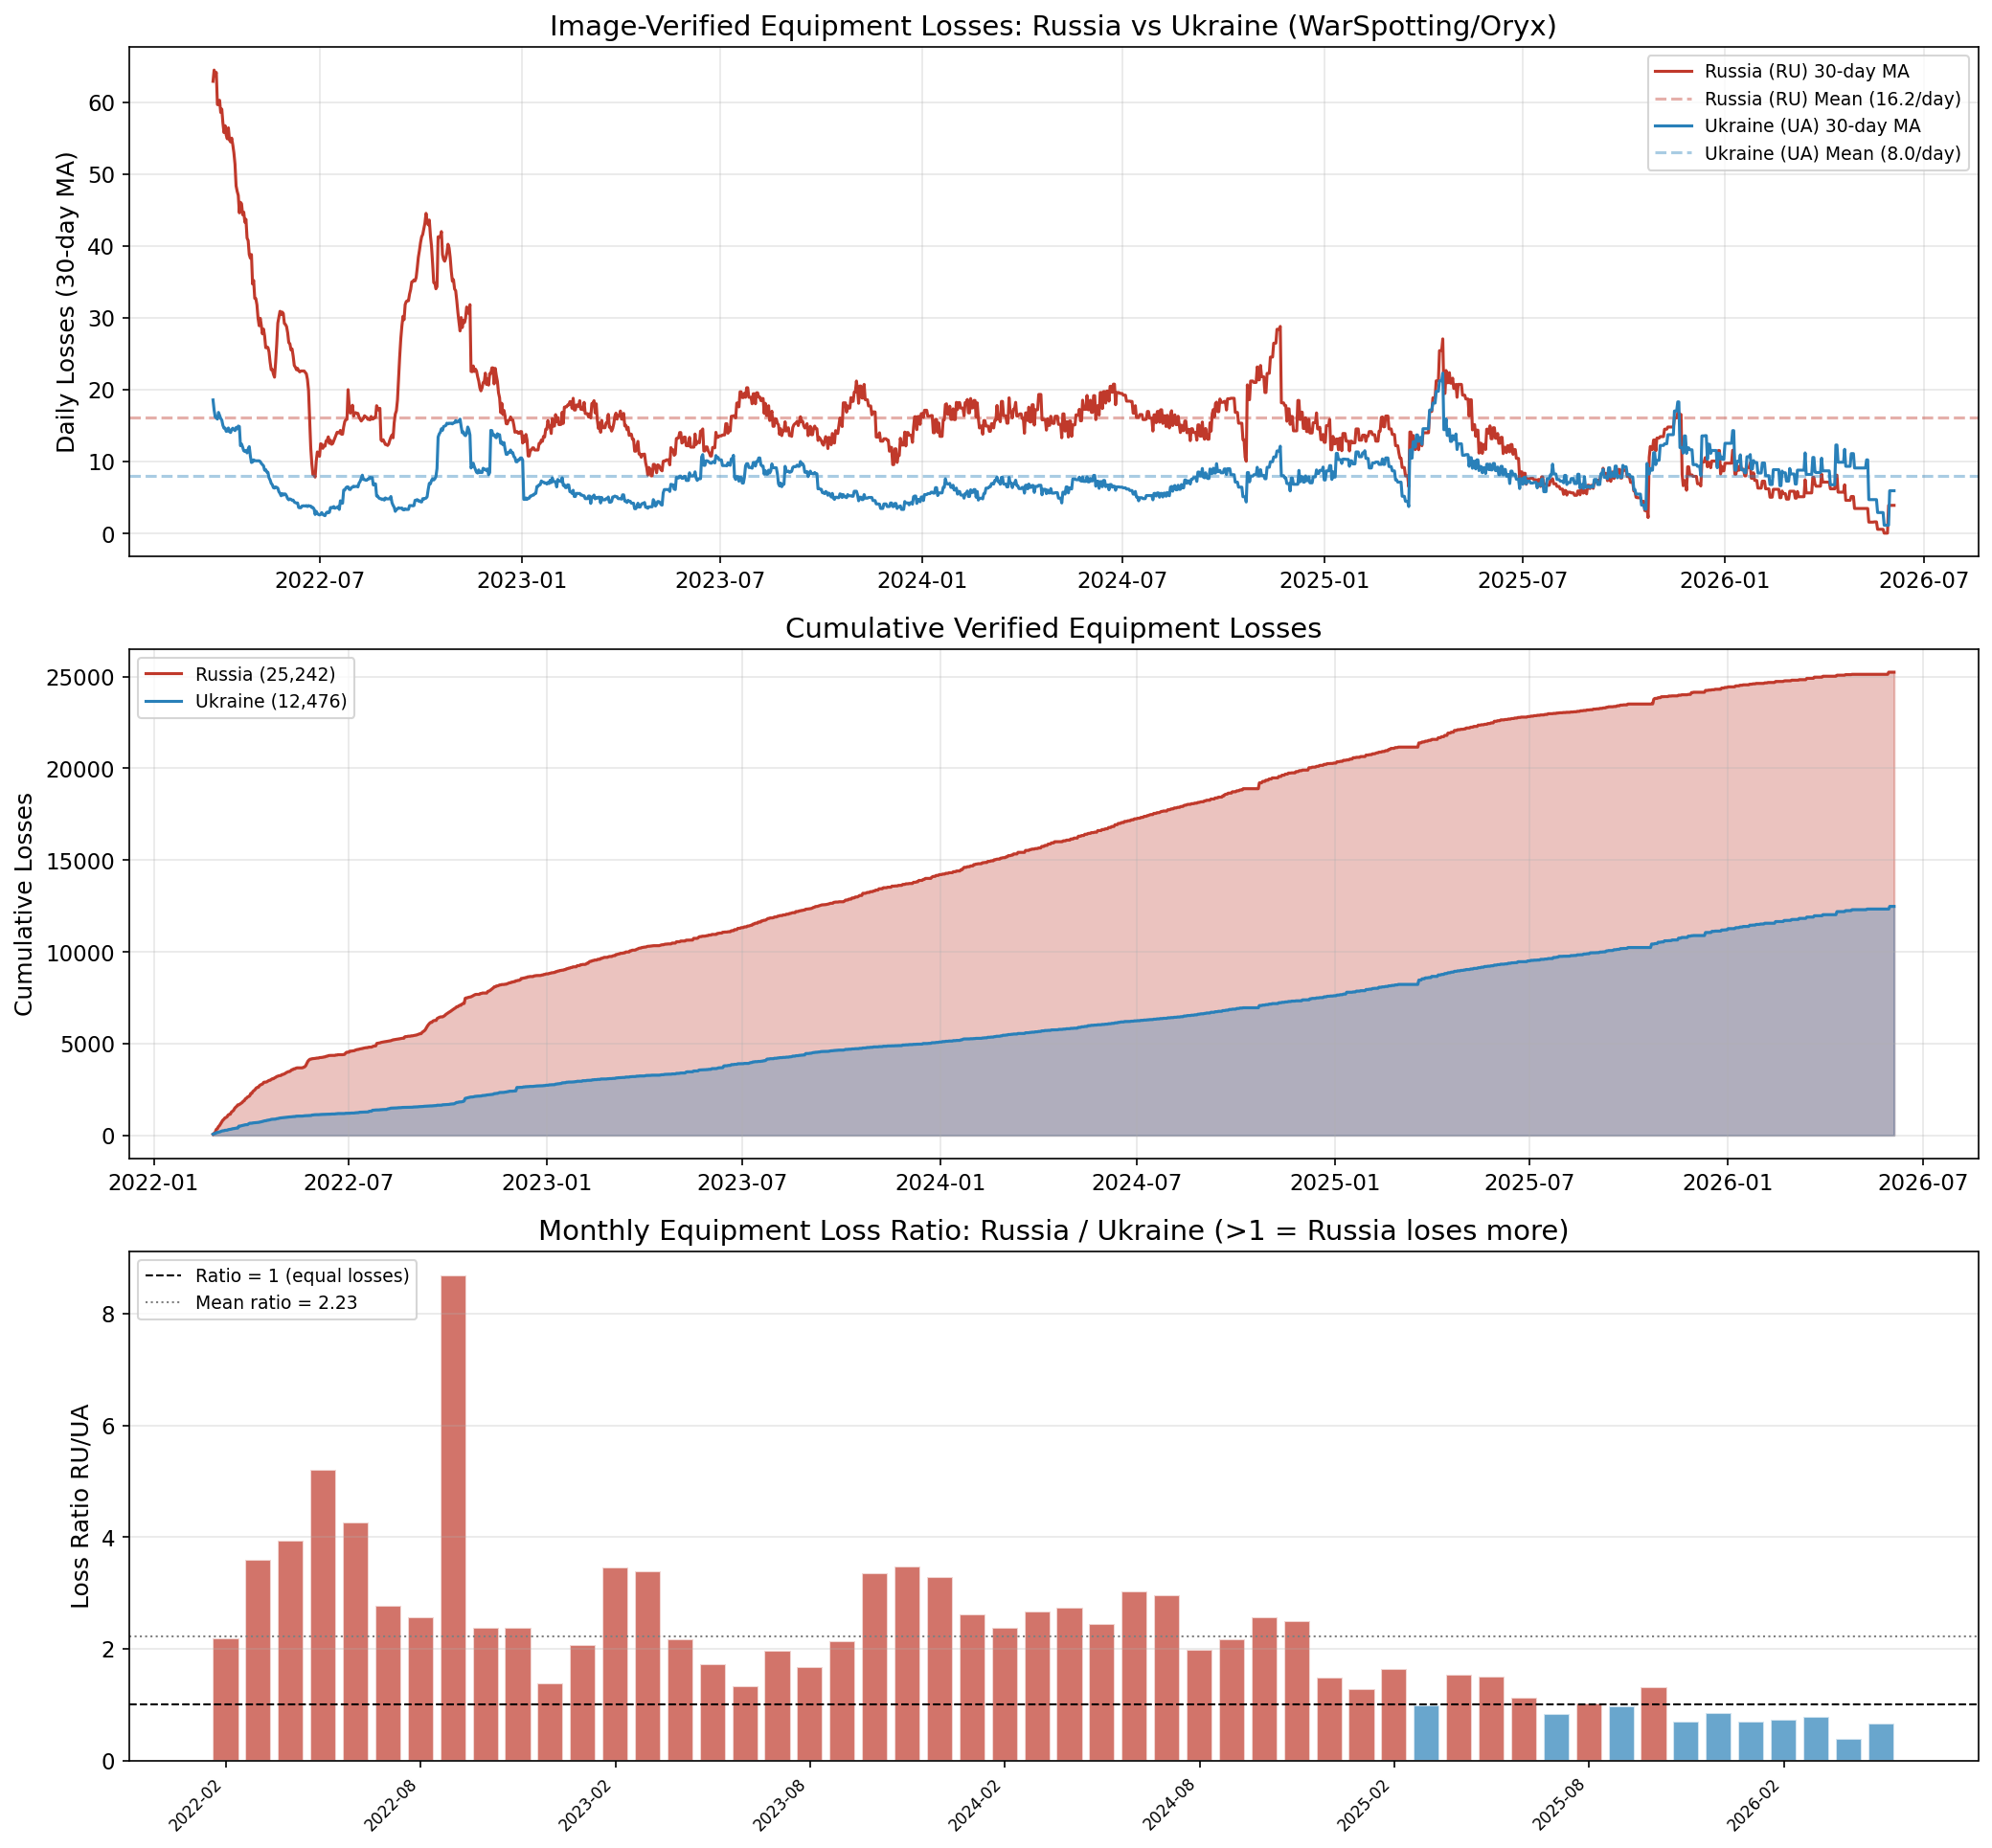
\includegraphics{../output/figures/10_both_sides_timeseries.png}
\caption{Daily and monthly Oryx loss trends for both sides.}
\label{fig:both-timeseries}
\end{figure}

\begin{figure}[htbp]
\centering
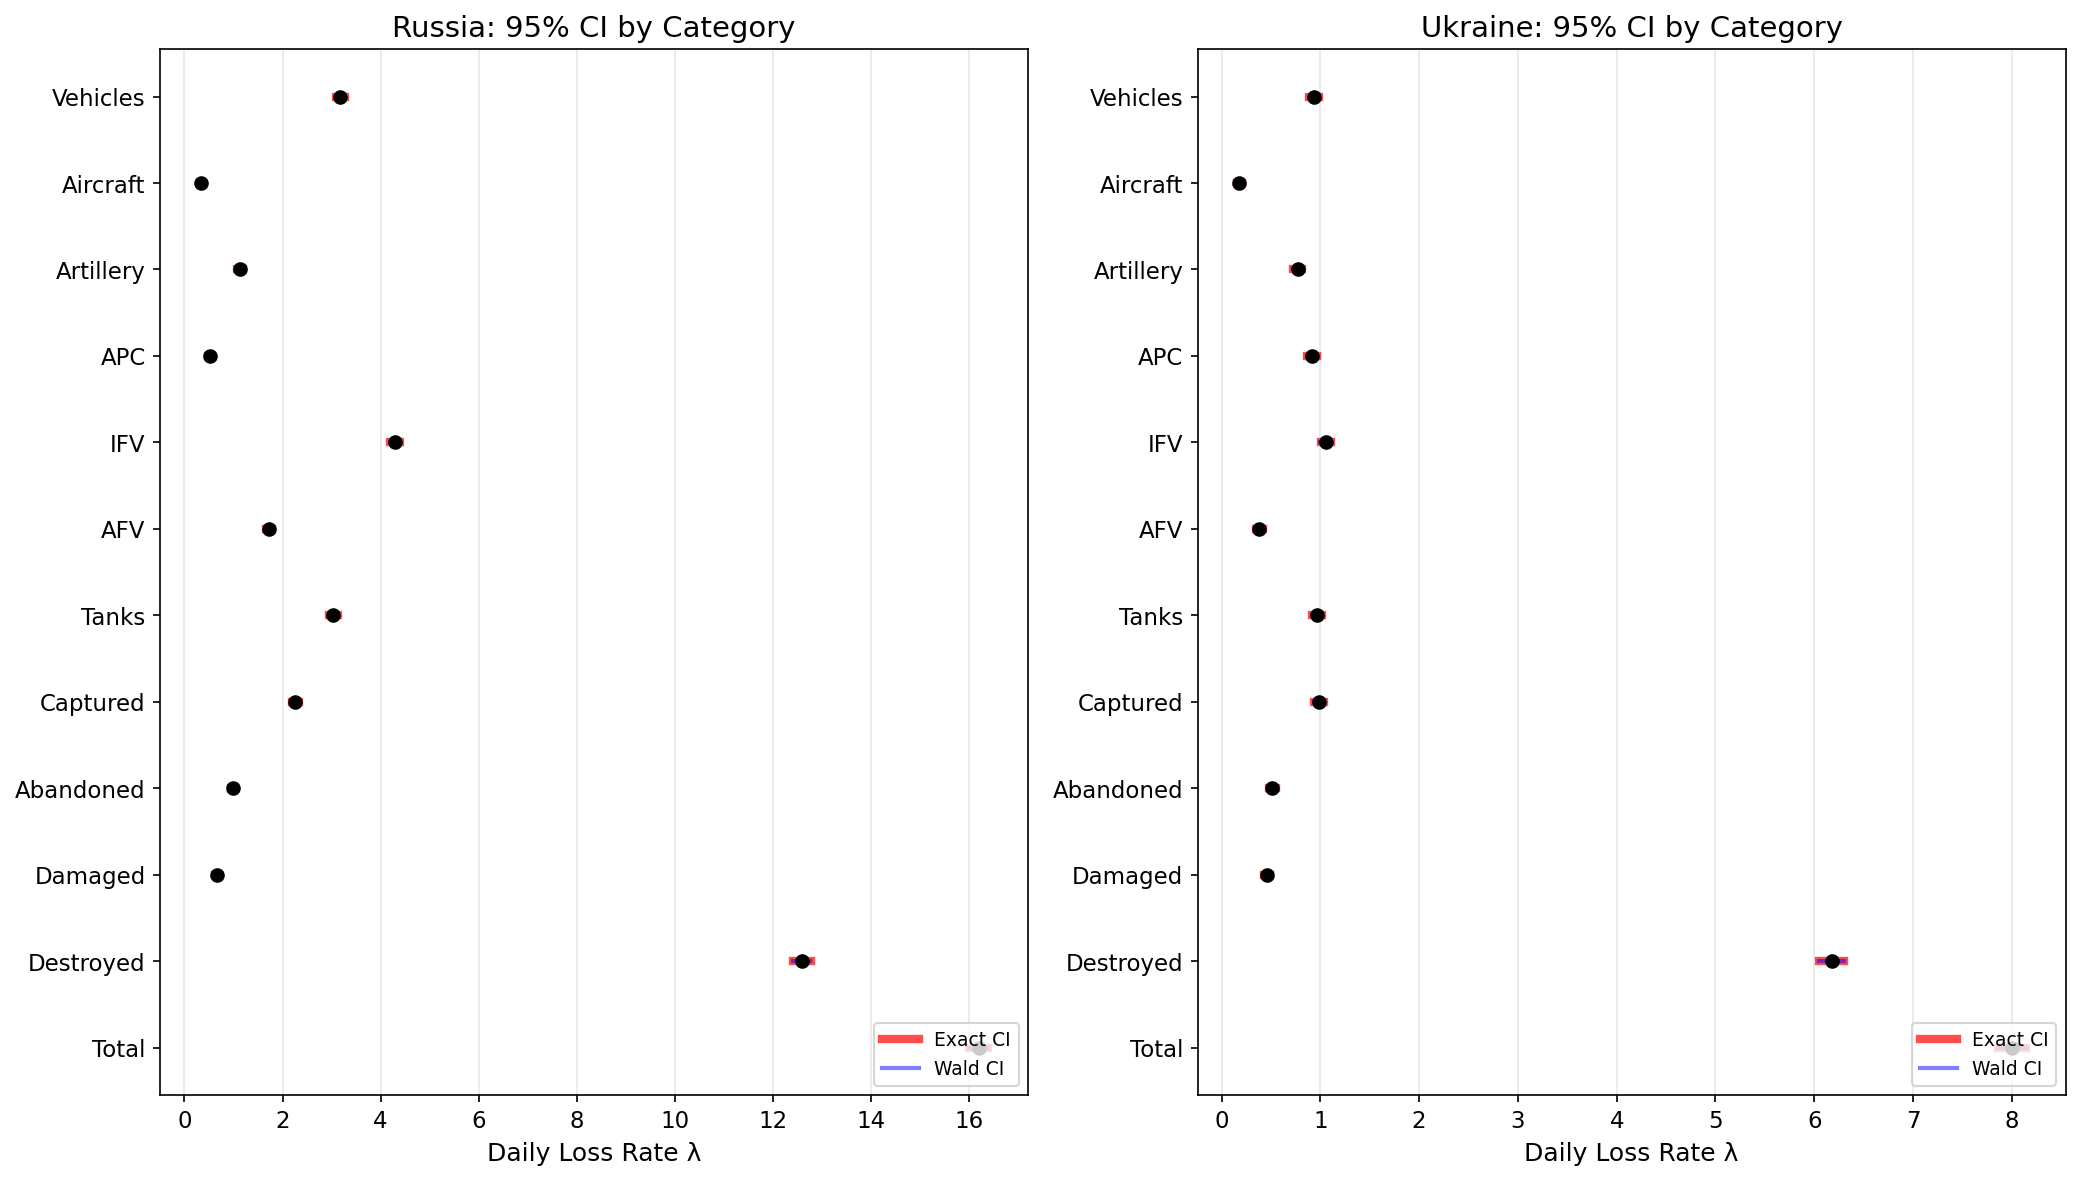
\includegraphics{../output/figures/11_both_sides_ci_forest.png}
\caption{Confidence intervals for verified daily loss rates of both sides.}
\label{fig:both-ci}
\end{figure}

\subsection{Monthly Dynamics}

Monthly aggregation reveals strong time variation. In the early phase from February to August 2022, the Russia-to-Ukraine ratio was above 3. During the Ukrainian counteroffensives of late 2022, the ratio declined toward 1.5--2.0. During 2023--2024, the ratio fluctuated around 1--2. In 2025--2026, several windows approached or fell below 1. If months affected by negative retroactive corrections are excluded, recent ratios are about 0.65--0.8; if all corrections are included, the weighted 2025--2026 ratio is about 0.96. The robust qualitative conclusion is that the verified loss-ratio advantage observed early in the war has narrowed sharply.

\subsection{Equipment-Type Comparisons}

\begin{longtable}{lrrrrr}
\toprule
Type & $\hat{\lambda}_{RU}$ & $\hat{\lambda}_{UA}$ & Ratio & E-test $p$ & Bonferroni \\
\midrule
\endhead
AFV & 1.720 & 0.383 & 4.49 & $<0.0001$ & *** \\
IFV & 4.298 & 1.052 & 4.08 & $<0.0001$ & *** \\
Vehicles & 3.174 & 0.934 & 3.40 & $<0.0001$ & *** \\
Tanks & 3.033 & 0.965 & 3.14 & $<0.0001$ & *** \\
Logistics & 0.702 & 0.251 & 2.80 & $<0.0001$ & *** \\
Engineering & 0.487 & 0.192 & 2.54 & $<0.0001$ & *** \\
Aircraft & 0.339 & 0.180 & 1.88 & $<0.0001$ & *** \\
Air defense & 0.387 & 0.253 & 1.53 & $<0.0001$ & *** \\
Artillery & 1.130 & 0.771 & 1.47 & $<0.0001$ & *** \\
\textbf{APC} & \textbf{0.516} & \textbf{0.914} & \textbf{0.56} & $<0.0001$ & *** \\
\bottomrule
\end{longtable}

All ten equipment-type comparisons remain significant after Bonferroni correction. Russia has especially high verified losses in offensive and maneuver equipment such as AFVs, IFVs, vehicles, and tanks. APC is the main reverse category, with higher verified Ukrainian losses. Figures~\ref{fig:type-compare} and \ref{fig:composition} visualize these patterns.

\begin{figure}[htbp]
\centering
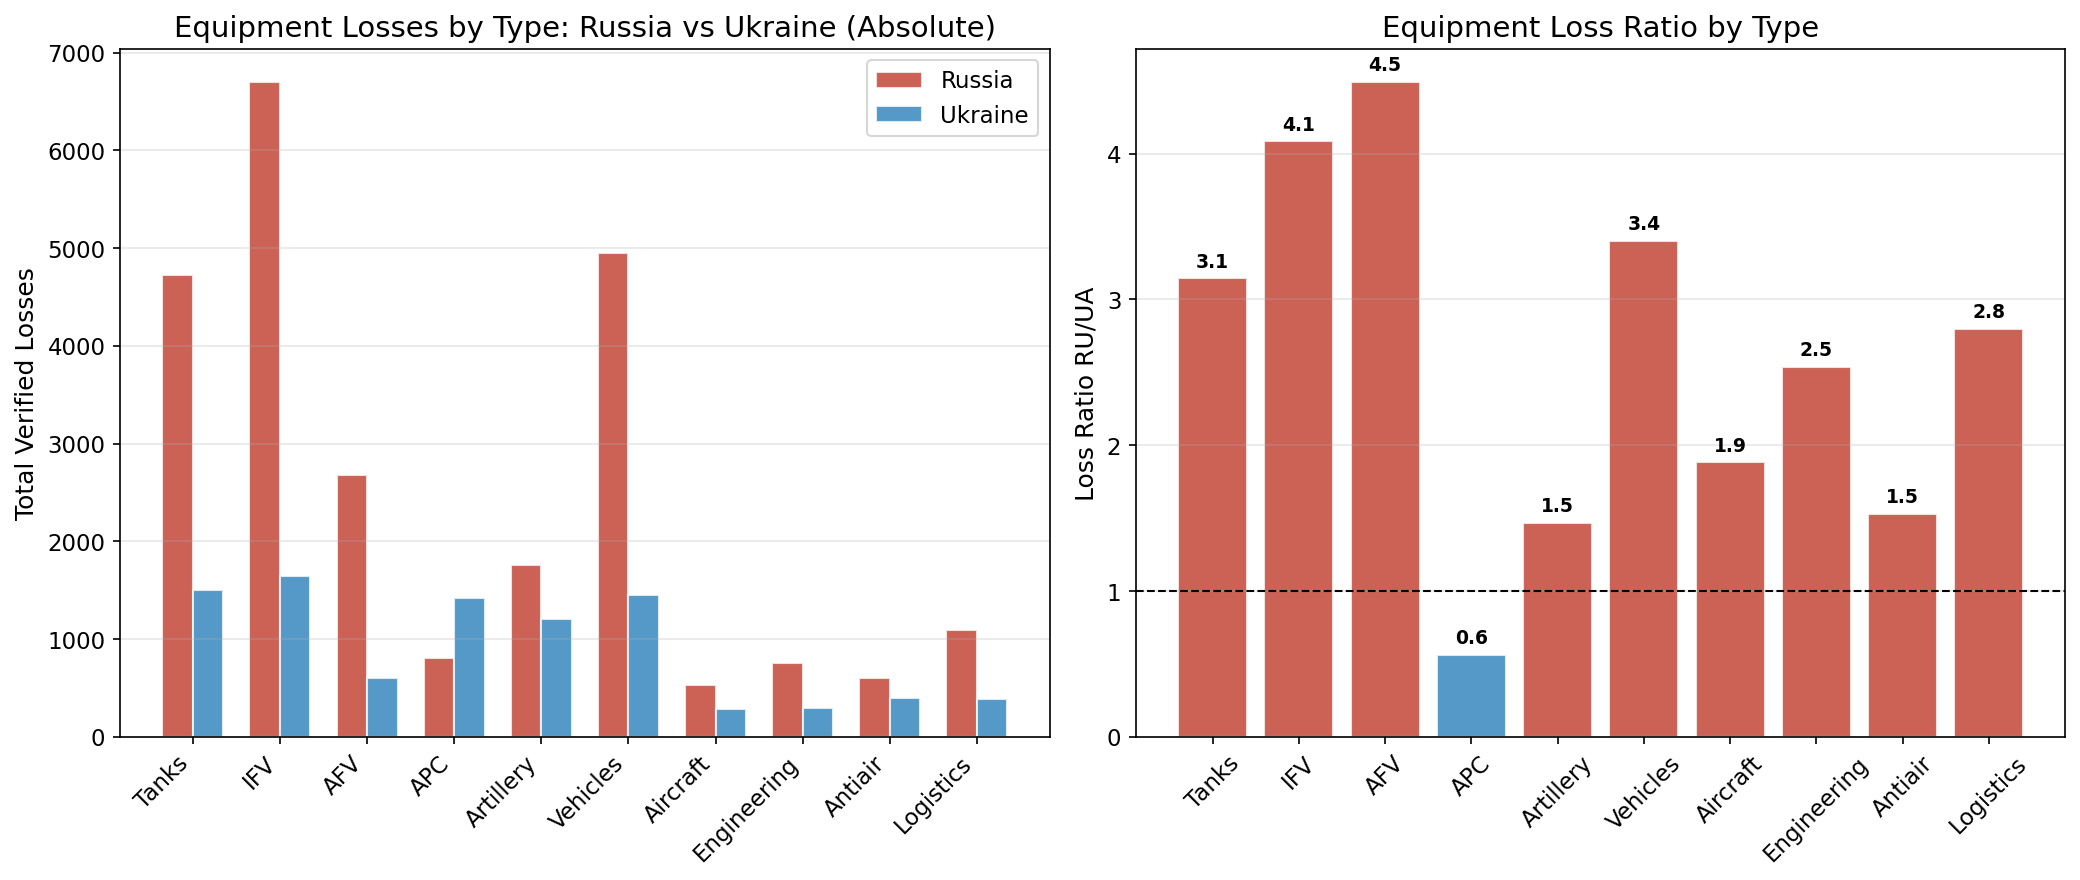
\includegraphics{../output/figures/12_equipment_type_comparison.png}
\caption{Equipment-type loss-rate comparison between Russia and Ukraine.}
\label{fig:type-compare}
\end{figure}

\begin{figure}[htbp]
\centering
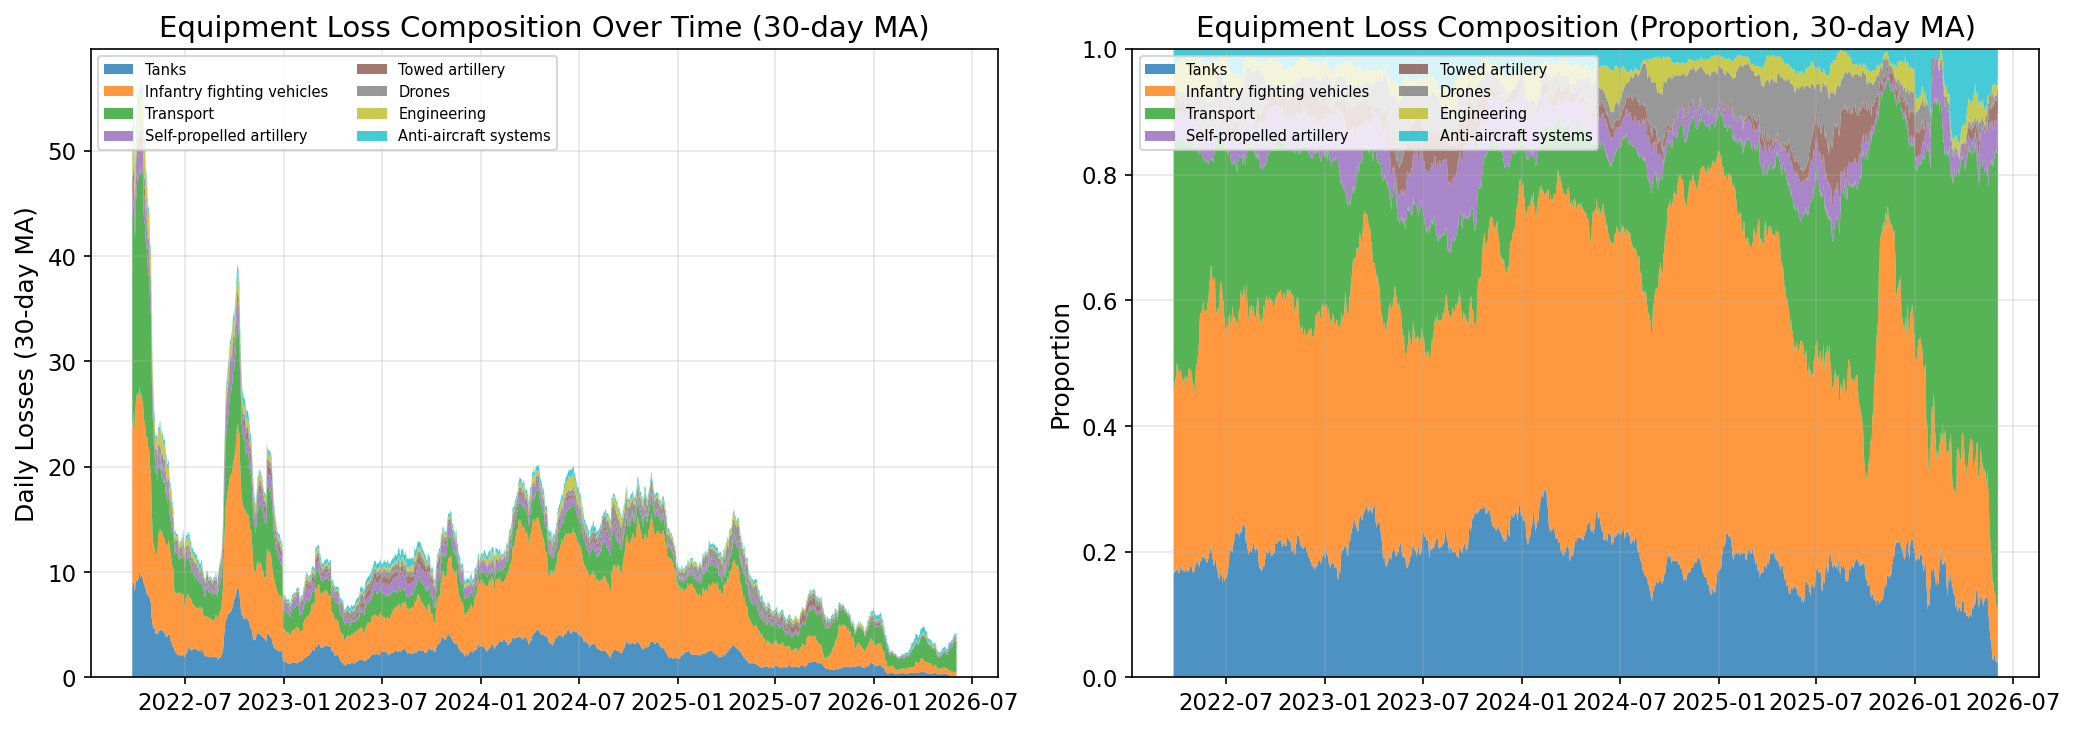
\includegraphics{../output/figures/05_equipment_composition.png}
\caption{Russian equipment-type composition in WarSpotting records.}
\label{fig:composition}
\end{figure}

\subsection{Loss Status}

\begin{longtable}{lrrrr}
\toprule
Status & $\hat{\lambda}_{RU}$ & $\hat{\lambda}_{UA}$ & Ratio & E-test $p$ \\
\midrule
\endhead
Destroyed & 12.59 & 6.17 & 2.04 & $<0.0001$ \\
Captured & 2.26 & 0.99 & 2.29 & $<0.0001$ \\
Abandoned & 0.99 & 0.51 & 1.93 & $<0.0001$ \\
Damaged & 0.66 & 0.46 & 1.44 & $<0.0001$ \\
\bottomrule
\end{longtable}

Destroyed equipment dominates both sides' verified records. Captured equipment is more prominent for Russia, consistent with episodes of withdrawal and abandonment. Figures~\ref{fig:status-pie} and \ref{fig:status-type} summarize these distributions.

\begin{figure}[htbp]
\centering
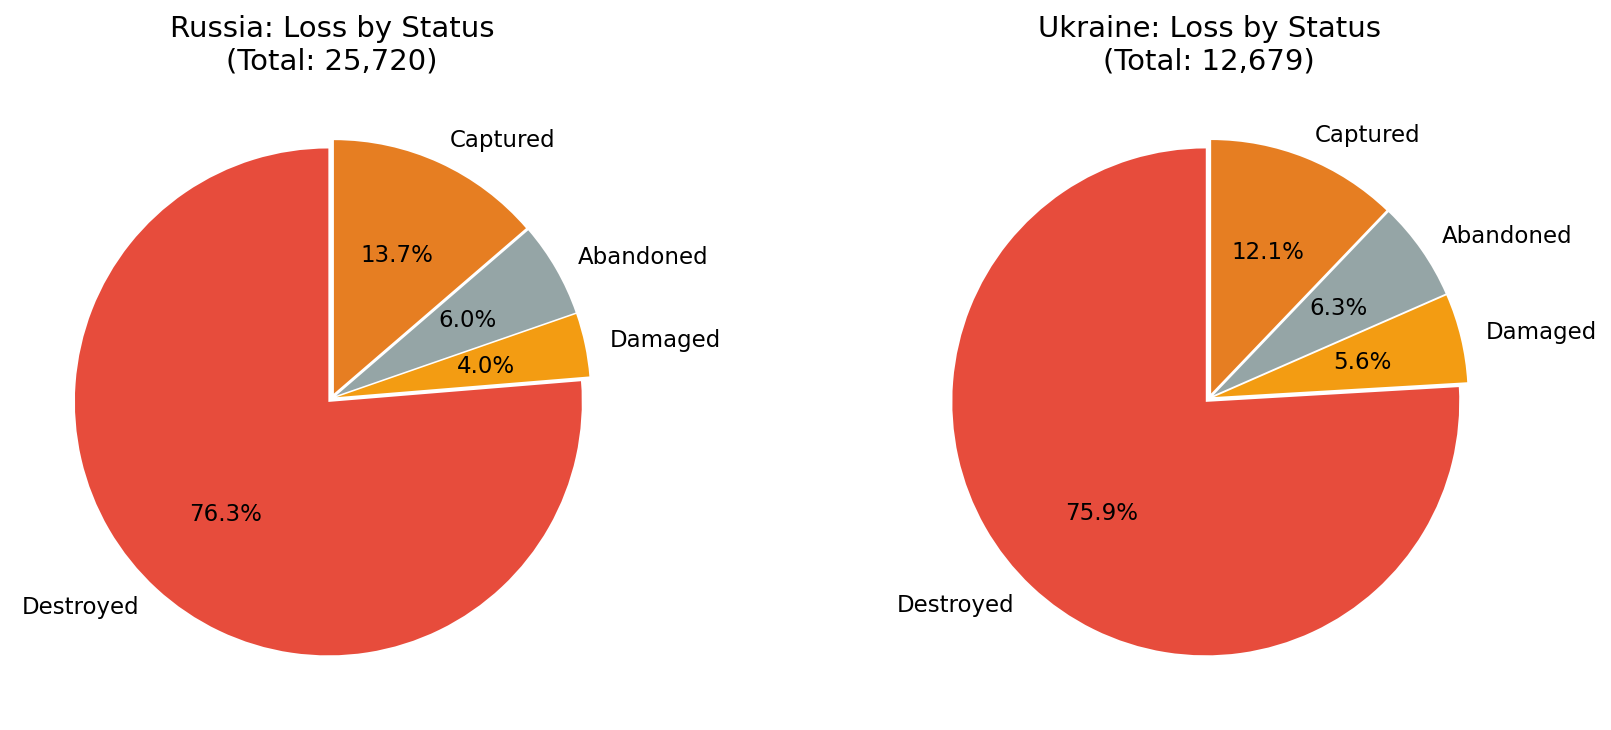
\includegraphics{../output/figures/13_both_sides_status_pie.png}
\caption{Loss-status composition for both sides.}
\label{fig:status-pie}
\end{figure}

\begin{figure}[htbp]
\centering
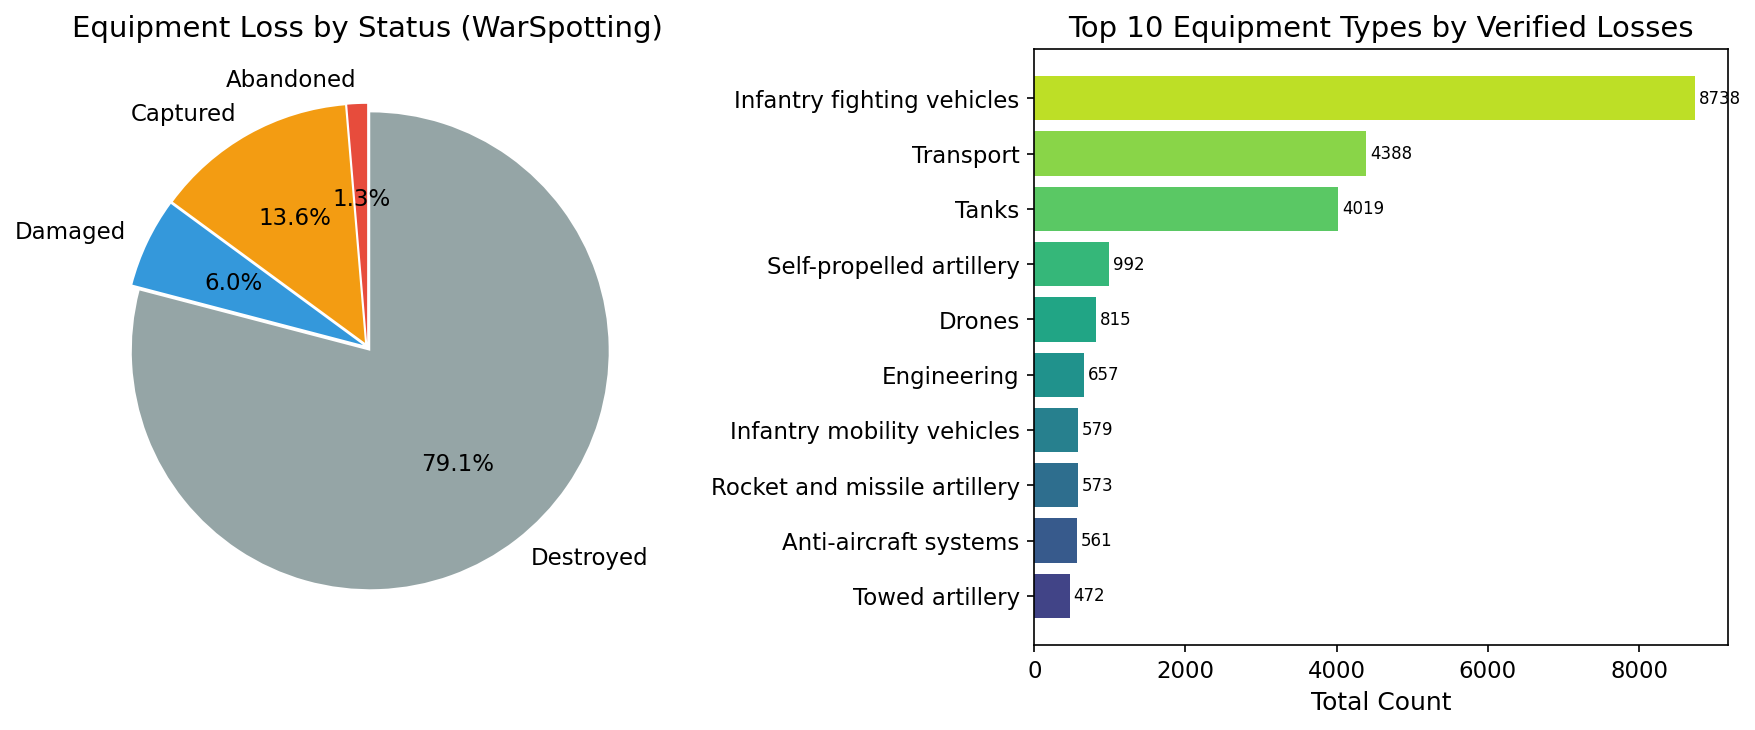
\includegraphics{../output/figures/09_status_and_type.png}
\caption{Russian loss status and equipment-type distribution in WarSpotting.}
\label{fig:status-type}
\end{figure}

\subsection{Confidence-Interval Coverage}

Monte Carlo simulations with $N=10{,}000$ replications and $n=30$ days evaluate coverage for $\lambda\in\{0.5,1,2,5,10,15,20,50\}$.

\begin{longtable}{lrrr}
\toprule
True $\lambda$ & Wald & Score & Exact \\
\midrule
\endhead
0.5 & \textbf{0.919} (low) & 0.951 & 0.966 \\
1.0 & 0.929 (low) & 0.946 & 0.957 \\
2.0 & 0.948 (slightly low) & 0.954 & 0.961 \\
5.0 & 0.955 & 0.956 & 0.956 \\
10.0 & 0.950 & 0.947 & 0.950 \\
15.0 & 0.949 & 0.949 & 0.953 \\
\bottomrule
\end{longtable}

Wald intervals under-cover for small rates, while Exact intervals maintain conservative coverage. For rare equipment categories, Exact intervals are therefore preferred. Figures~\ref{fig:ci-forest}--\ref{fig:qq} show interval estimates, interval-width comparisons, and Poisson Q-Q diagnostics.

\begin{figure}[htbp]
\centering
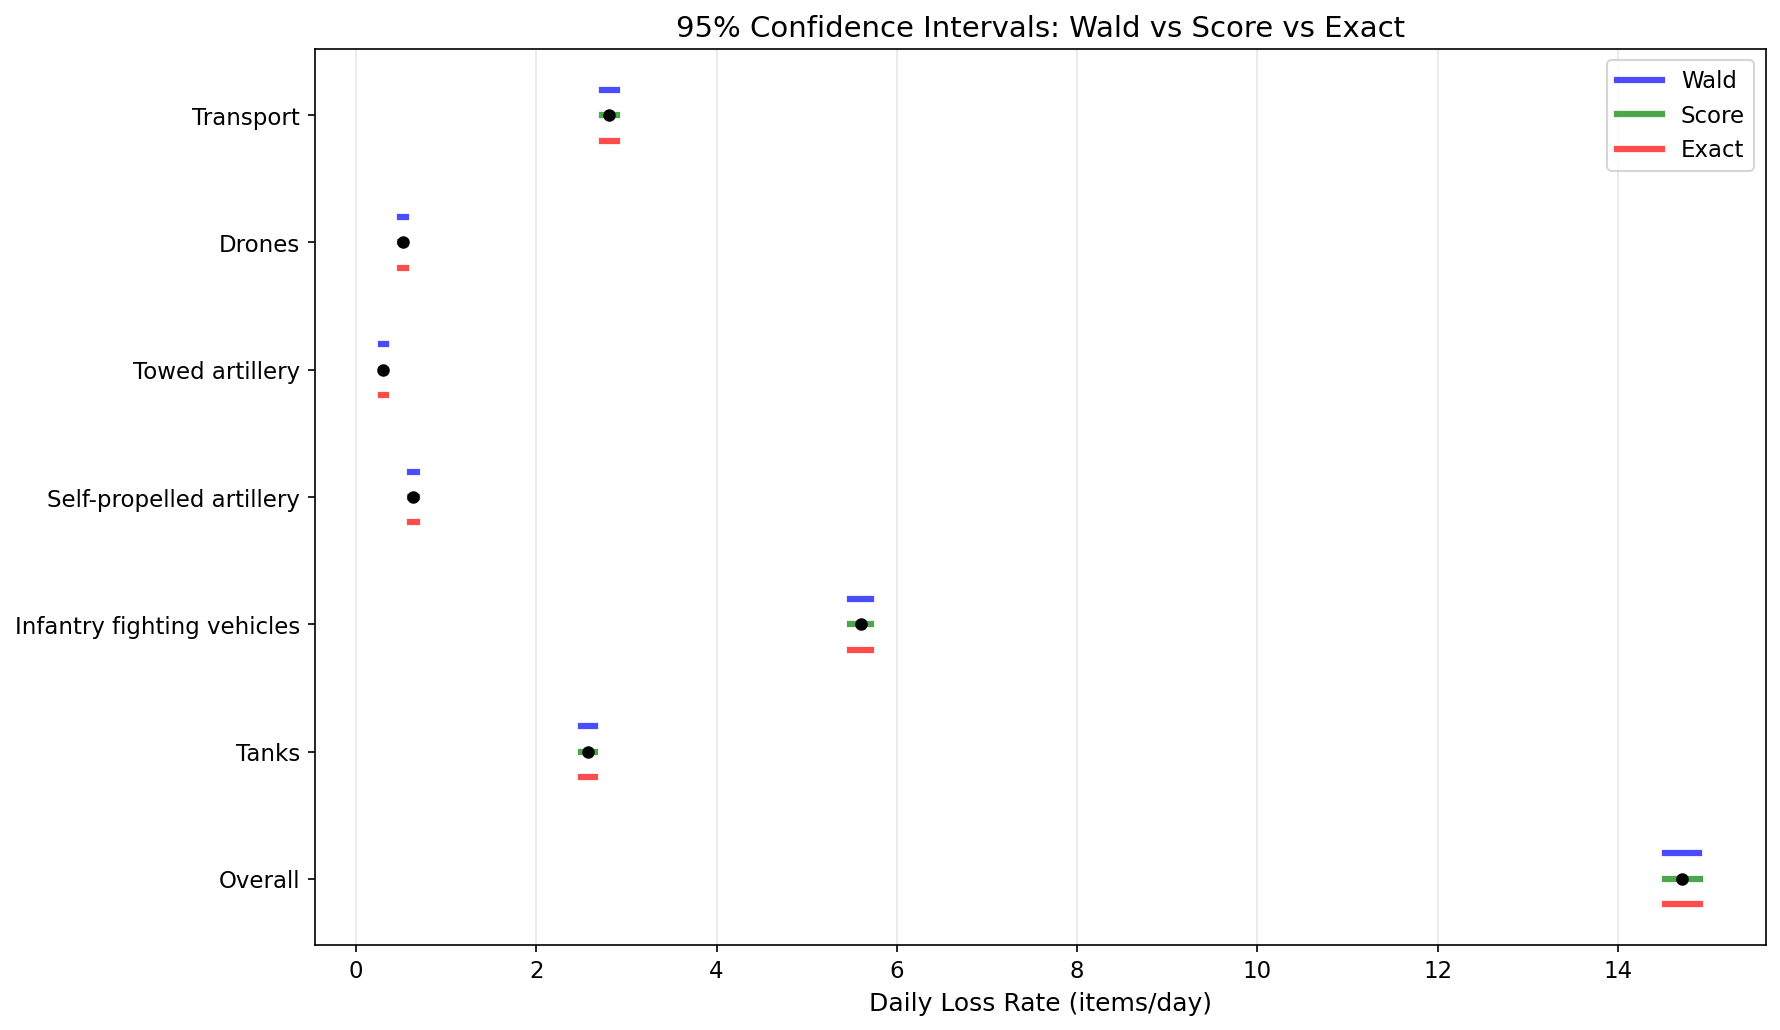
\includegraphics{../output/figures/03_ci_forest_plot.png}
\caption{Poisson confidence-interval forest plot.}
\label{fig:ci-forest}
\end{figure}

\begin{figure}[htbp]
\centering
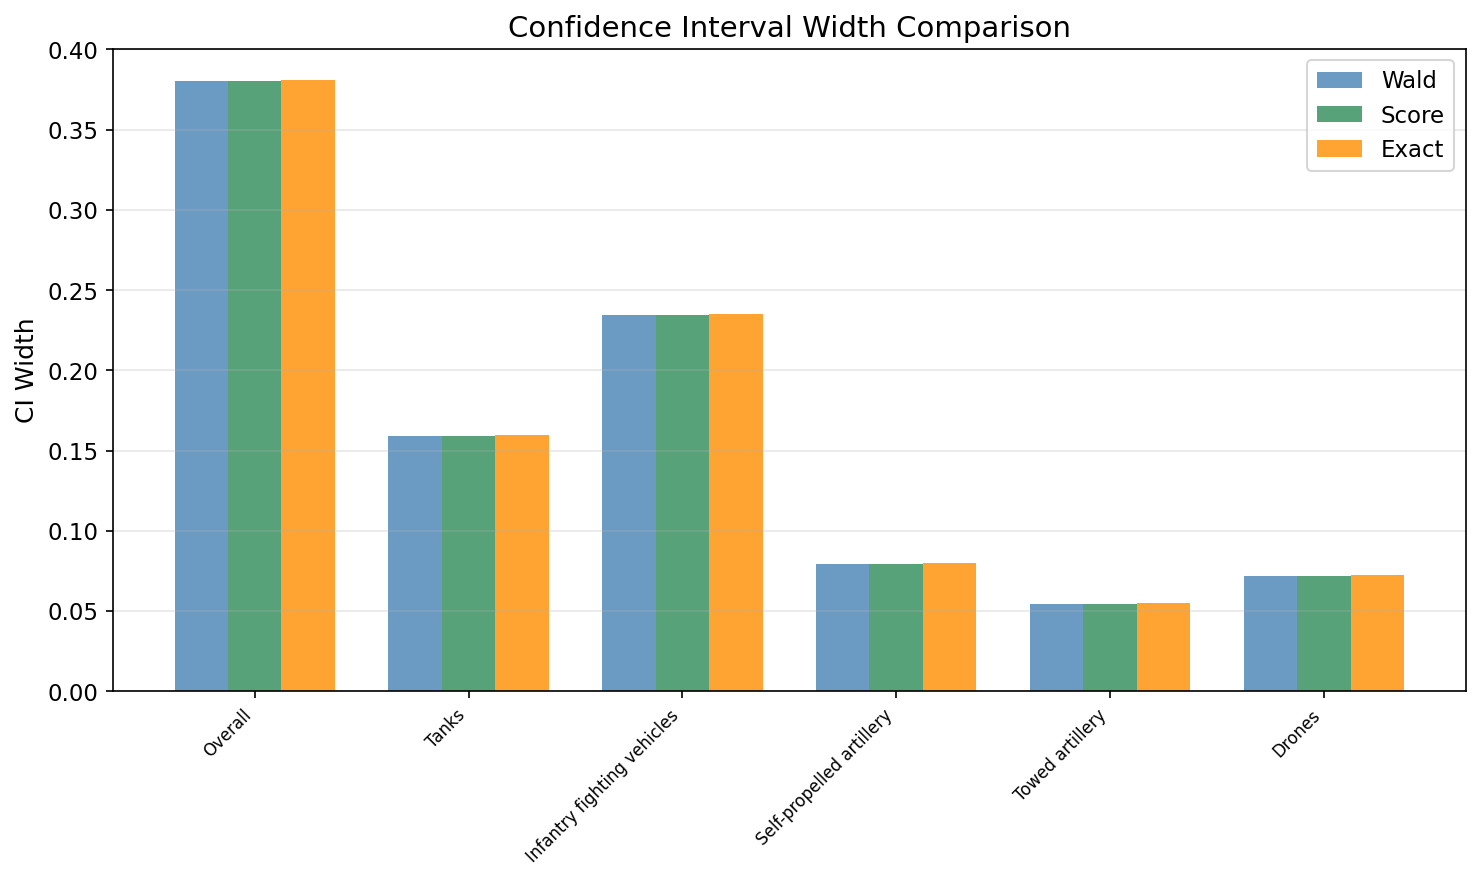
\includegraphics{../output/figures/07_ci_width_comparison.png}
\caption{Interval-width comparison across confidence-interval methods.}
\label{fig:ci-width}
\end{figure}

\begin{figure}[htbp]
\centering
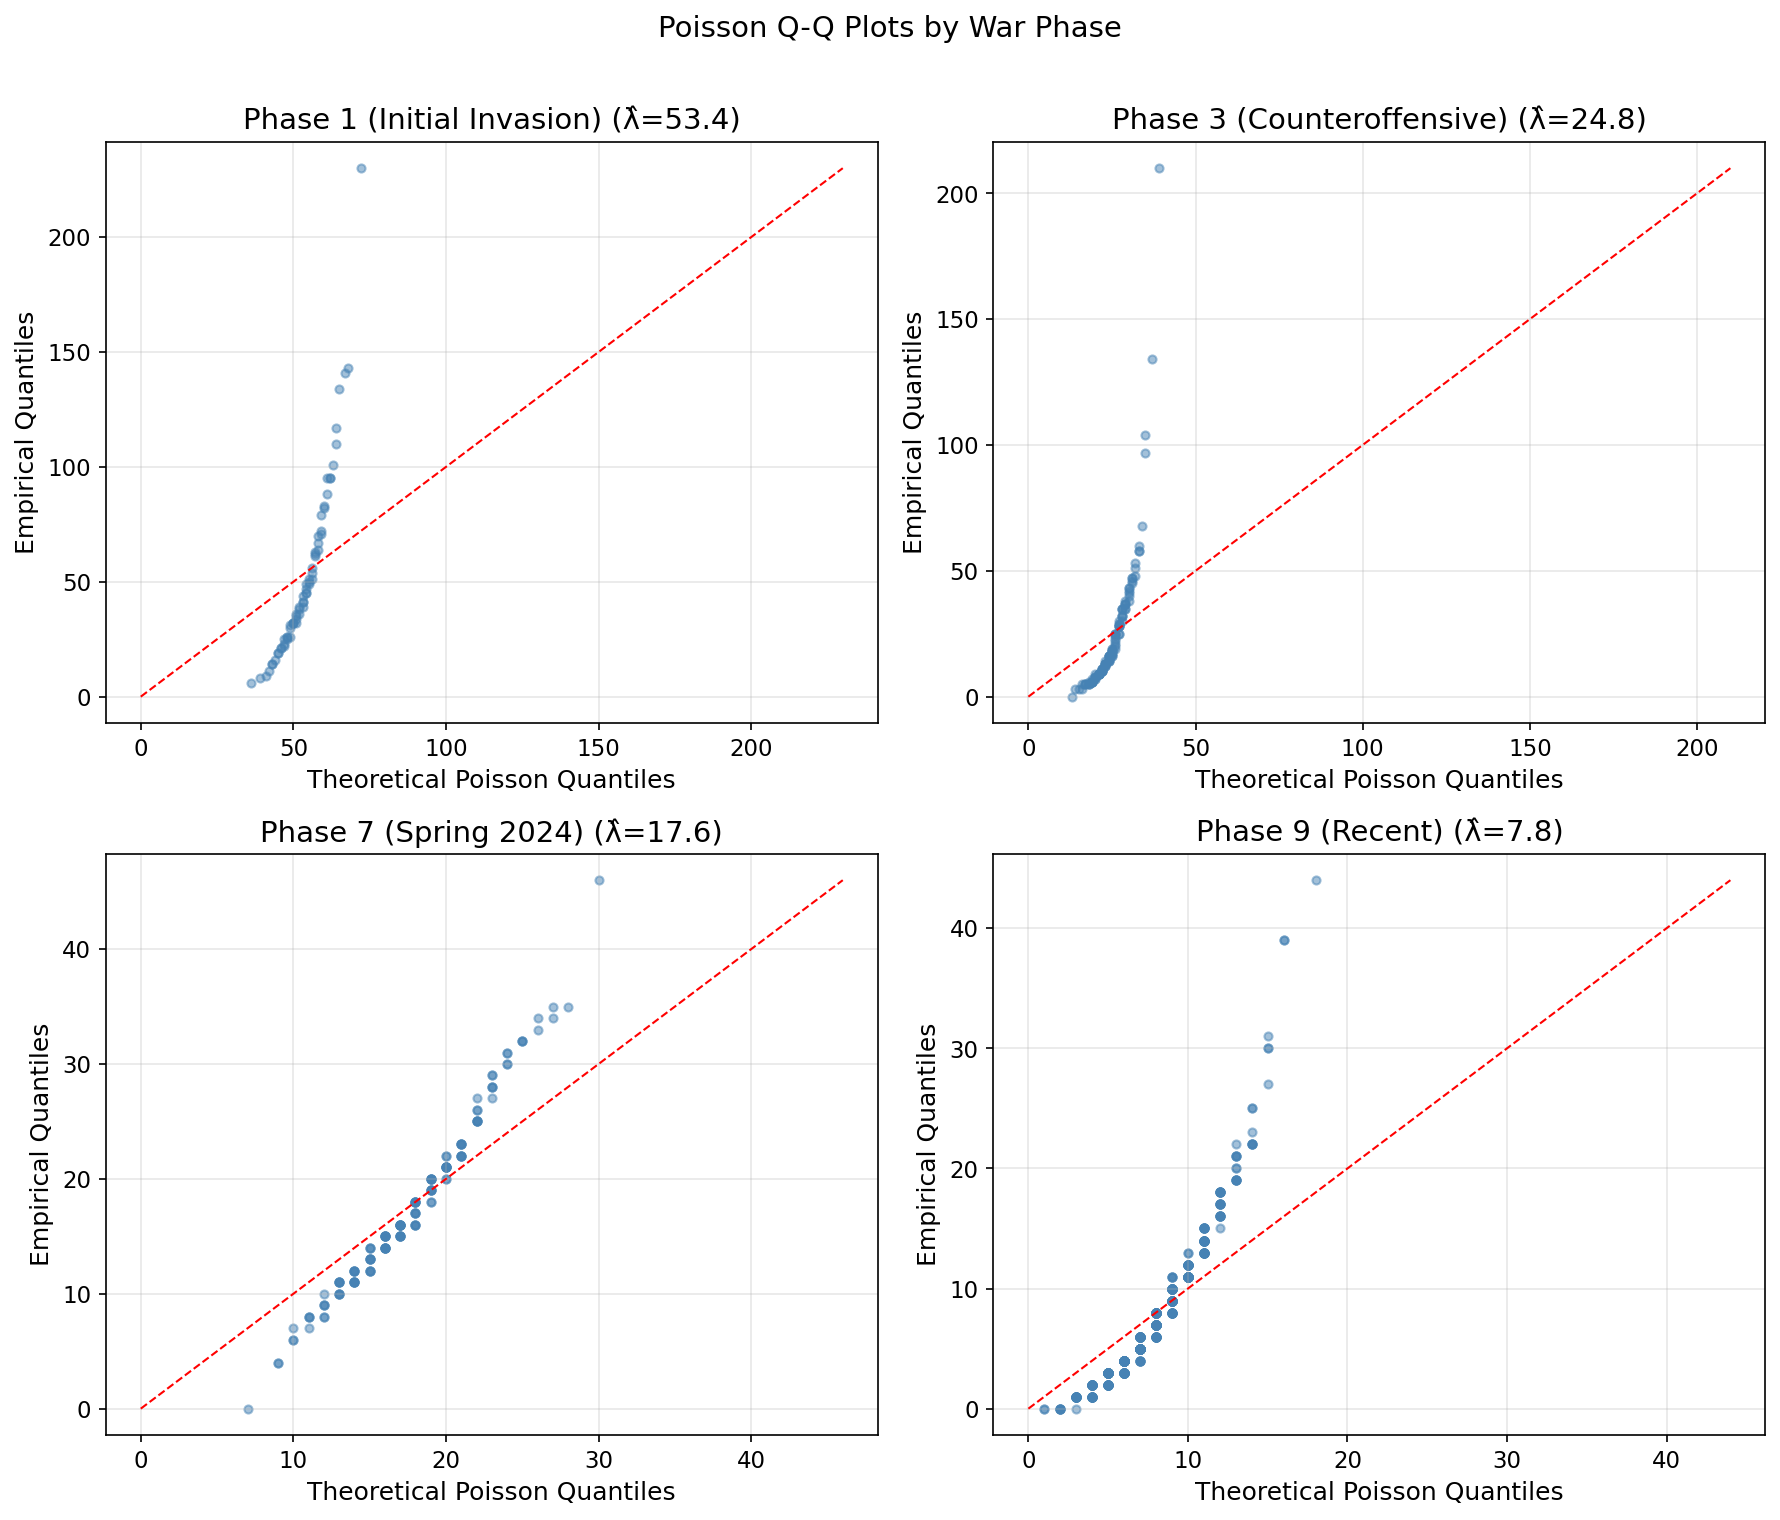
\includegraphics{../output/figures/06_poisson_qqplot.png}
\caption{Poisson Q-Q diagnostic plot.}
\label{fig:qq}
\end{figure}

\subsection{Block Bootstrap}

\begin{longtable}{lrr}
\toprule
Method & Bootstrap SE & 95\% interval \\
\midrule
\endhead
IID Bootstrap ($b=1$) & 0.42 & [13.91, 15.54] \\
Block Bootstrap ($b=11$) & \textbf{0.99} & [12.82, 16.59] \\
BCa Block Bootstrap ($b=11$) & --- & [13.18, 17.29] \\
\bottomrule
\end{longtable}

The block-bootstrap standard error is about 2.4 times the IID bootstrap value. Ignoring temporal dependence therefore understates uncertainty by more than half. Figure~\ref{fig:bootstrap} shows the broader block-bootstrap distribution.

\begin{figure}[htbp]
\centering
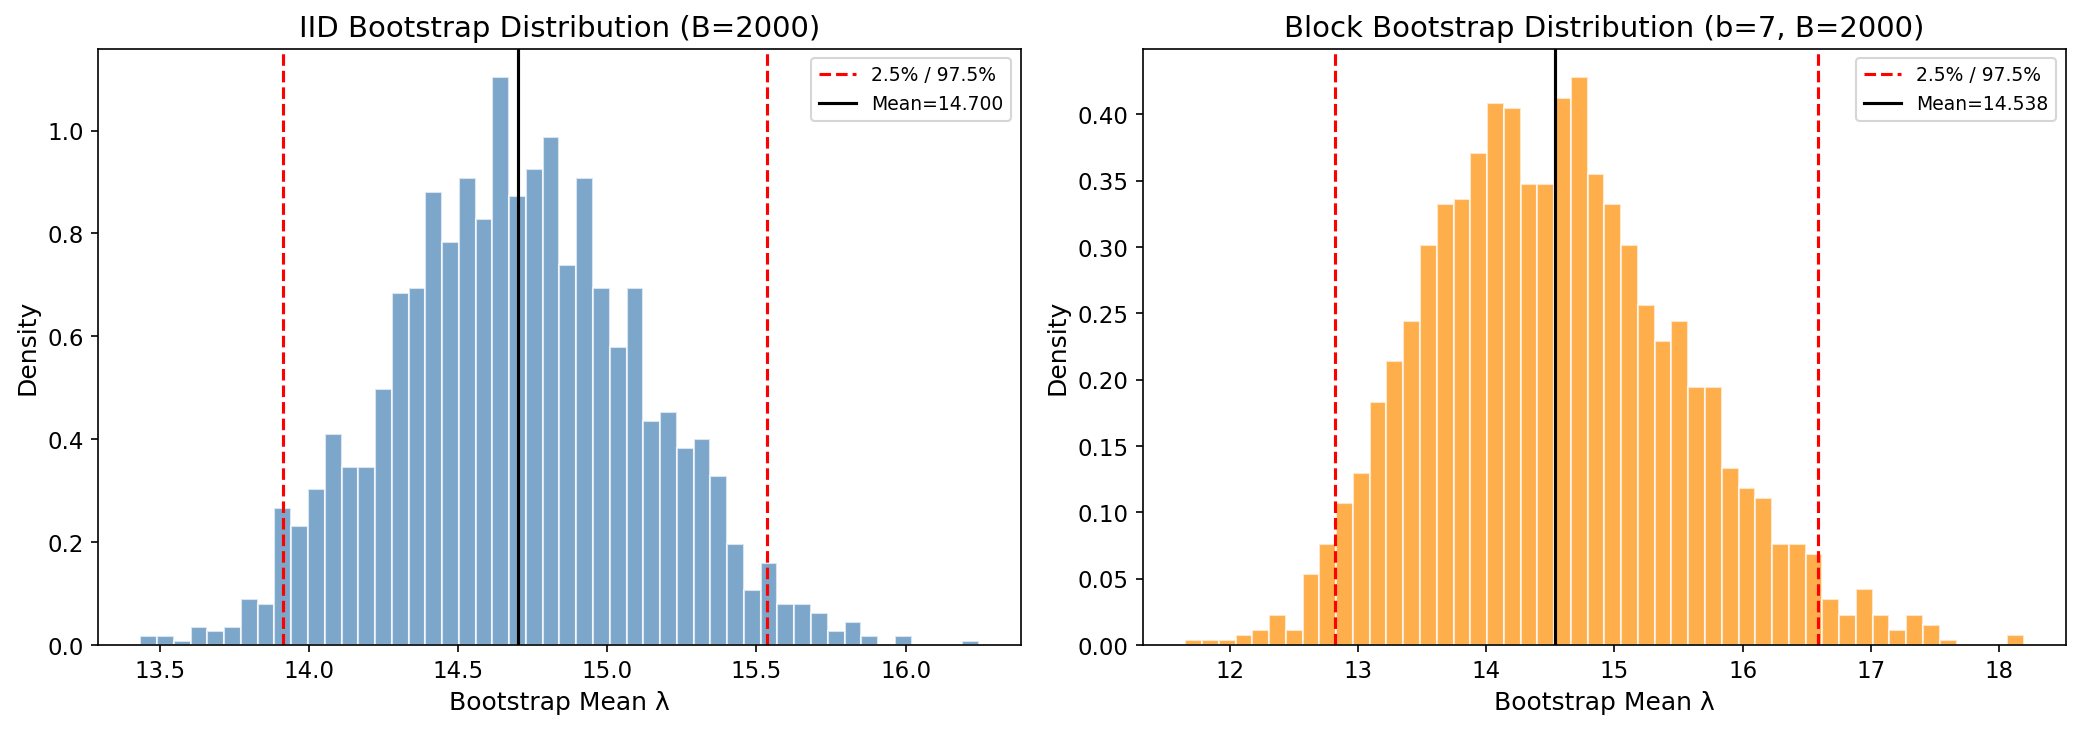
\includegraphics{../output/figures/04_bootstrap_distribution.png}
\caption{IID Bootstrap and Moving Block Bootstrap distributions.}
\label{fig:bootstrap}
\end{figure}

\subsection{War Phases}

\begin{longtable}{lrrr}
\toprule
Phase & Daily $\hat{\lambda}$ & SE & Days \\
\midrule
\endhead
Phase 1 (2022.2--4), initial invasion & 53.38 & 0.90 & 66 \\
Phase 3 (2022.9--12), Ukrainian counteroffensive & 24.75 & 0.45 & 122 \\
Phase 7 (2024.3--7), spring offensive & 17.65 & 0.34 & 153 \\
Phase 9 (2025.1--2026.6), recent period & 7.79 & 0.12 & 519 \\
\bottomrule
\end{longtable}

A likelihood-ratio test strongly rejects equal phase means ($LR=8919.0$, $df=8$, $p<0.0001$). The early-war verified loss level is much higher than the recent level. Figures~\ref{fig:daily} and \ref{fig:phase-box} show the phase structure.

\begin{figure}[htbp]
\centering
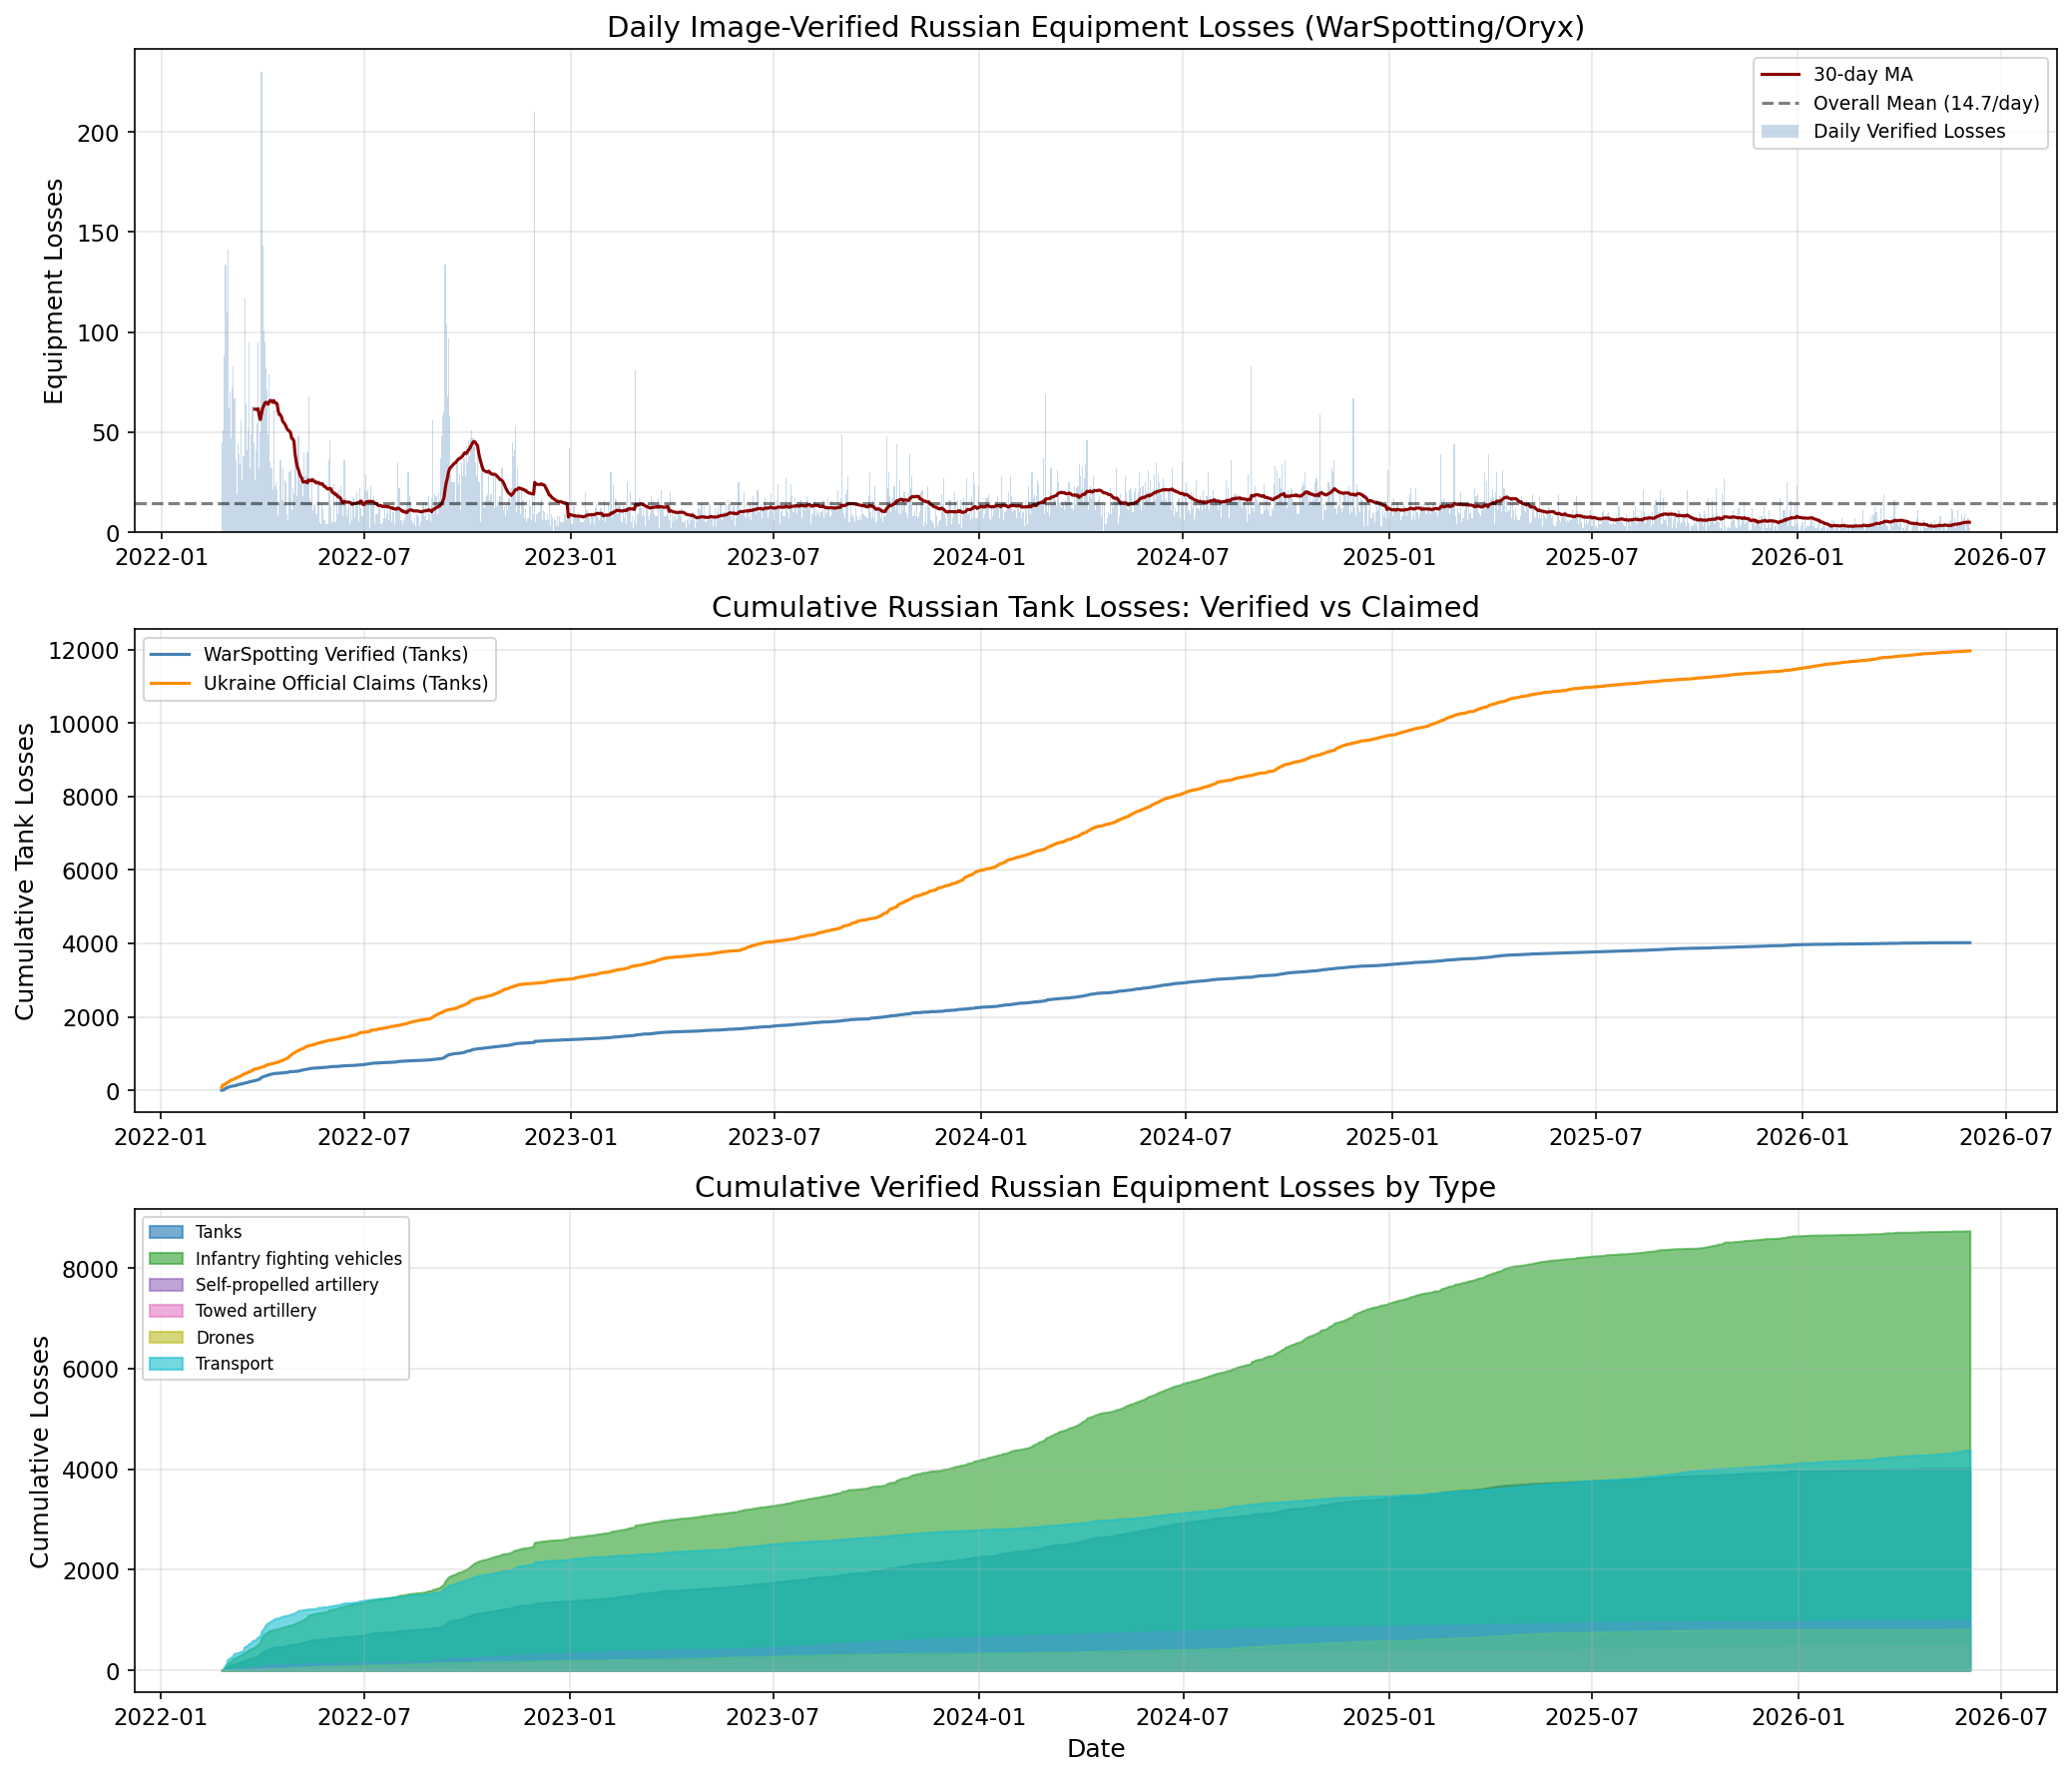
\includegraphics{../output/figures/01_daily_loss_timeseries.png}
\caption{Russian daily verified loss time series from WarSpotting.}
\label{fig:daily}
\end{figure}

\begin{figure}[htbp]
\centering
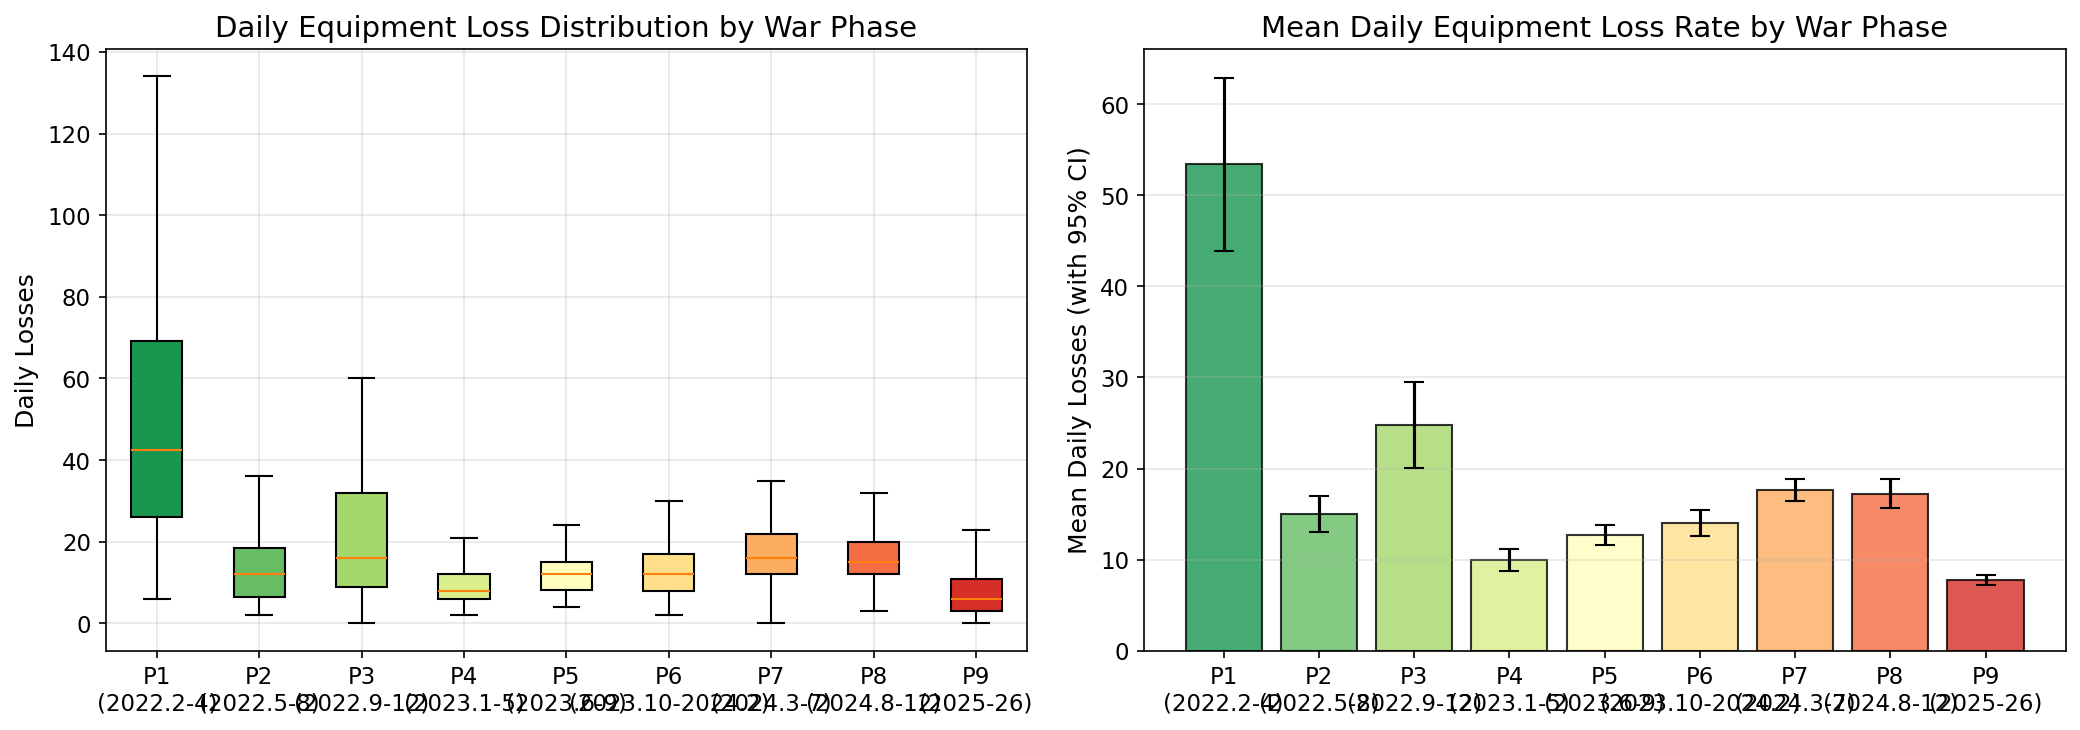
\includegraphics{../output/figures/02_phase_boxplot.png}
\caption{Daily loss distributions by war phase.}
\label{fig:phase-box}
\end{figure}

\subsection{Official Claims versus Verified Losses}

\begin{longtable}{lrrrr}
\toprule
Equipment & Verified rate & Claimed rate & Claim/verified ratio & E-test $p$ \\
\midrule
\endhead
Tanks & 2.57 & 7.68 & \textbf{2.98} & $<0.0001$ \\
Armoured vehicles & 5.60 & 15.85 & \textbf{2.83} & $<0.0001$ \\
Artillery & 0.94 & 27.62 & \textbf{29.44} & $<0.0001$ \\
\bottomrule
\end{longtable}

Official claims substantially exceed visually verified counts. The artillery ratio is especially large, likely reflecting both verification difficulty and differences in definitions such as suppressed or damaged positions versus destroyed systems. Figure~\ref{fig:claims} shows the divergence between official and verified series.

\begin{figure}[htbp]
\centering
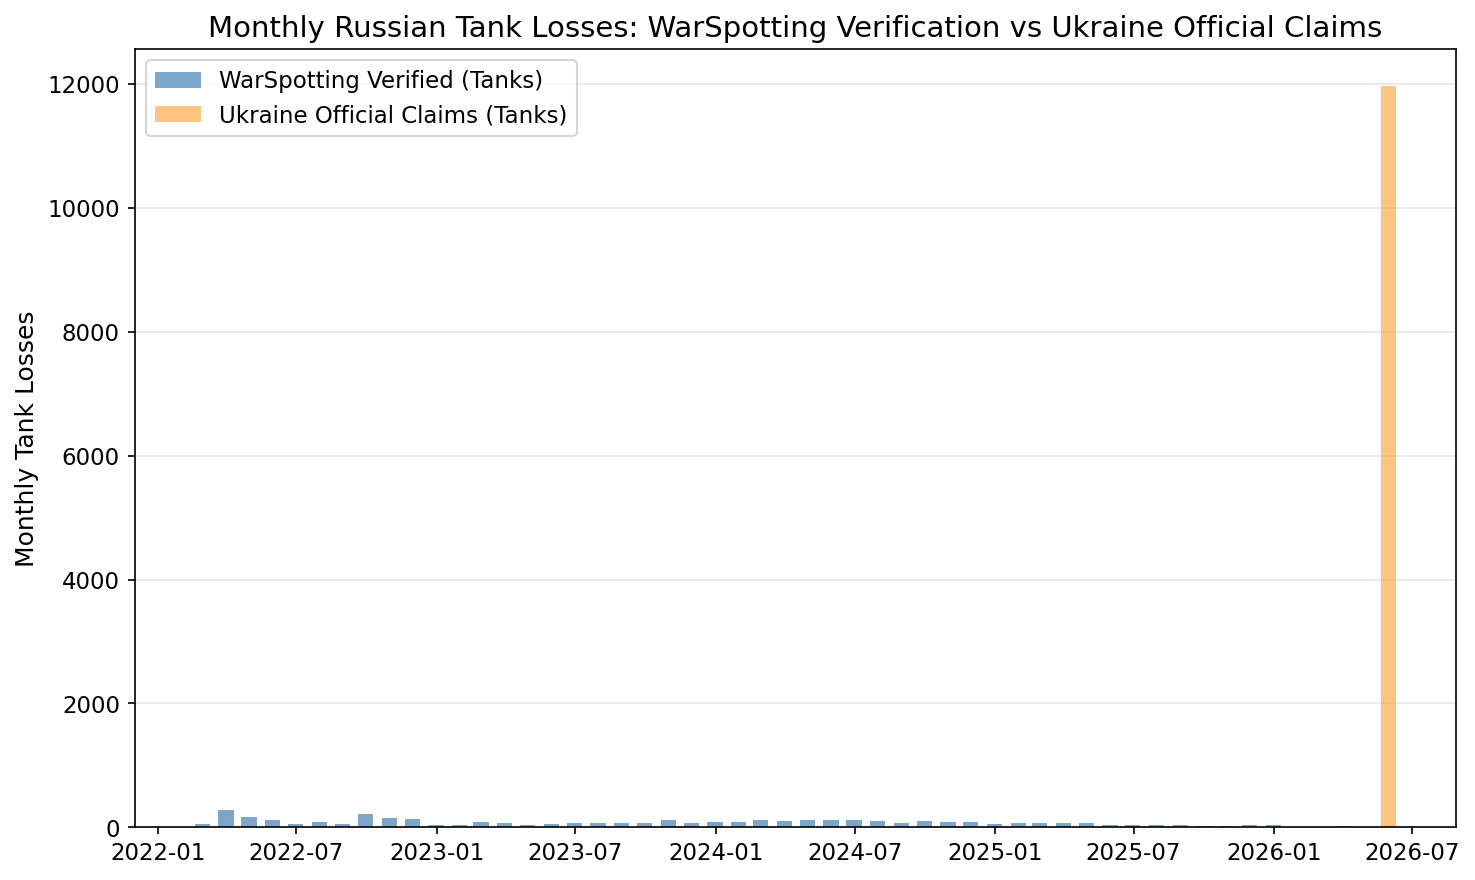
\includegraphics{../output/figures/08_claims_vs_verified.png}
\caption{Ukrainian official claims versus WarSpotting verified records.}
\label{fig:claims}
\end{figure}

\clearpage

\subsection{Bias-Corrected Rate-Ratio Inference}

The observed rate ratio is about 2.06--2.07. A reversal of the conclusion $\rho_{\mathrm{true}}>1$ would require
\[
\frac{p_{UA}}{p_{RU}} < \frac{1}{2.06}\approx 0.485.
\]
Thus, Ukrainian losses would need to be observed at less than half the Russian observation probability for the rate-ratio conclusion to reverse.

\begin{longtable}{lrrrr}
\toprule
Scenario & $p_{RU}$ range & $p_{UA}$ range & $\rho_{\mathrm{true}}$ range & Still $>1$? \\
\midrule
\endhead
Conservative, large visibility gap & [0.8, 0.9] & [0.4, 0.5] & [0.92, 1.29] & Borderline \\
Moderate, plausible assumption & [0.7, 0.8] & [0.5, 0.7] & [1.29, 2.06] & Yes \\
Optimistic, small visibility gap & [0.5, 0.7] & [0.6, 0.8] & [1.77, 3.30] & Yes \\
\bottomrule
\end{longtable}

Embedding $p_{RU}\sim\mathrm{Beta}(7,3)$ and $p_{UA}\sim\mathrm{Beta}(5.5,4.5)$ into the block-bootstrap procedure yields a bias-corrected median rate ratio of 1.63 and a 95\% interval of [0.67, 3.44]. Under these priors, $P(\rho_{\mathrm{corrected}}>1)=88.1\%$. The conclusion is therefore directionally robust but not entirely identified from Oryx data alone. Figure~\ref{fig:sensitivity} displays the sensitivity surface.

\begin{figure}[htbp]
\centering
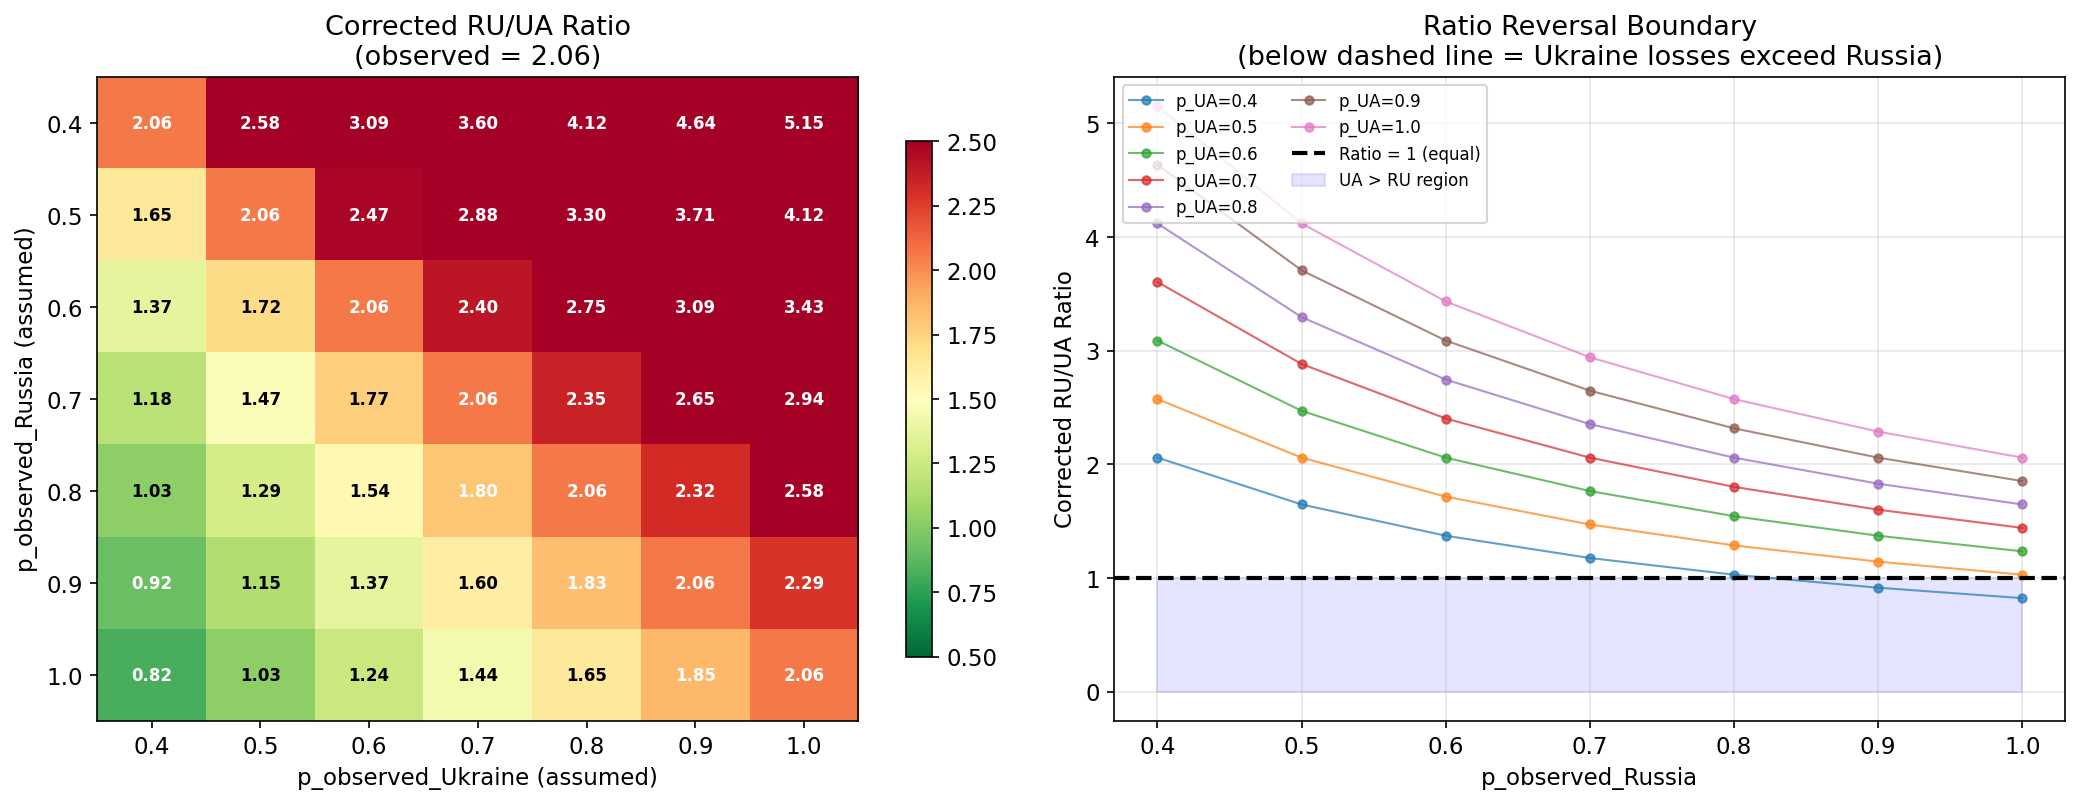
\includegraphics{../output/figures/15_sensitivity_heatmap.png}
\caption{Sensitivity of the corrected rate ratio to observation probabilities.}
\label{fig:sensitivity}
\end{figure}

\subsection{Spatial Distribution}

WarSpotting contains coordinates for 14,066 Russian loss records, about 61.2\% of the item-level dataset. The eastern theater, especially Donetsk, dominates the spatial distribution. The hottest one-degree grid cell, approximately $(48^\circ N,37^\circ E)$ around the Pokrovsk direction, contains 3,019 losses, or 21.5\% of geocoded losses. The top three Donetsk-region grid cells together account for about 45.1\%. Figure~\ref{fig:spatial} shows the spatial concentration.

\begin{figure}[htbp]
\centering
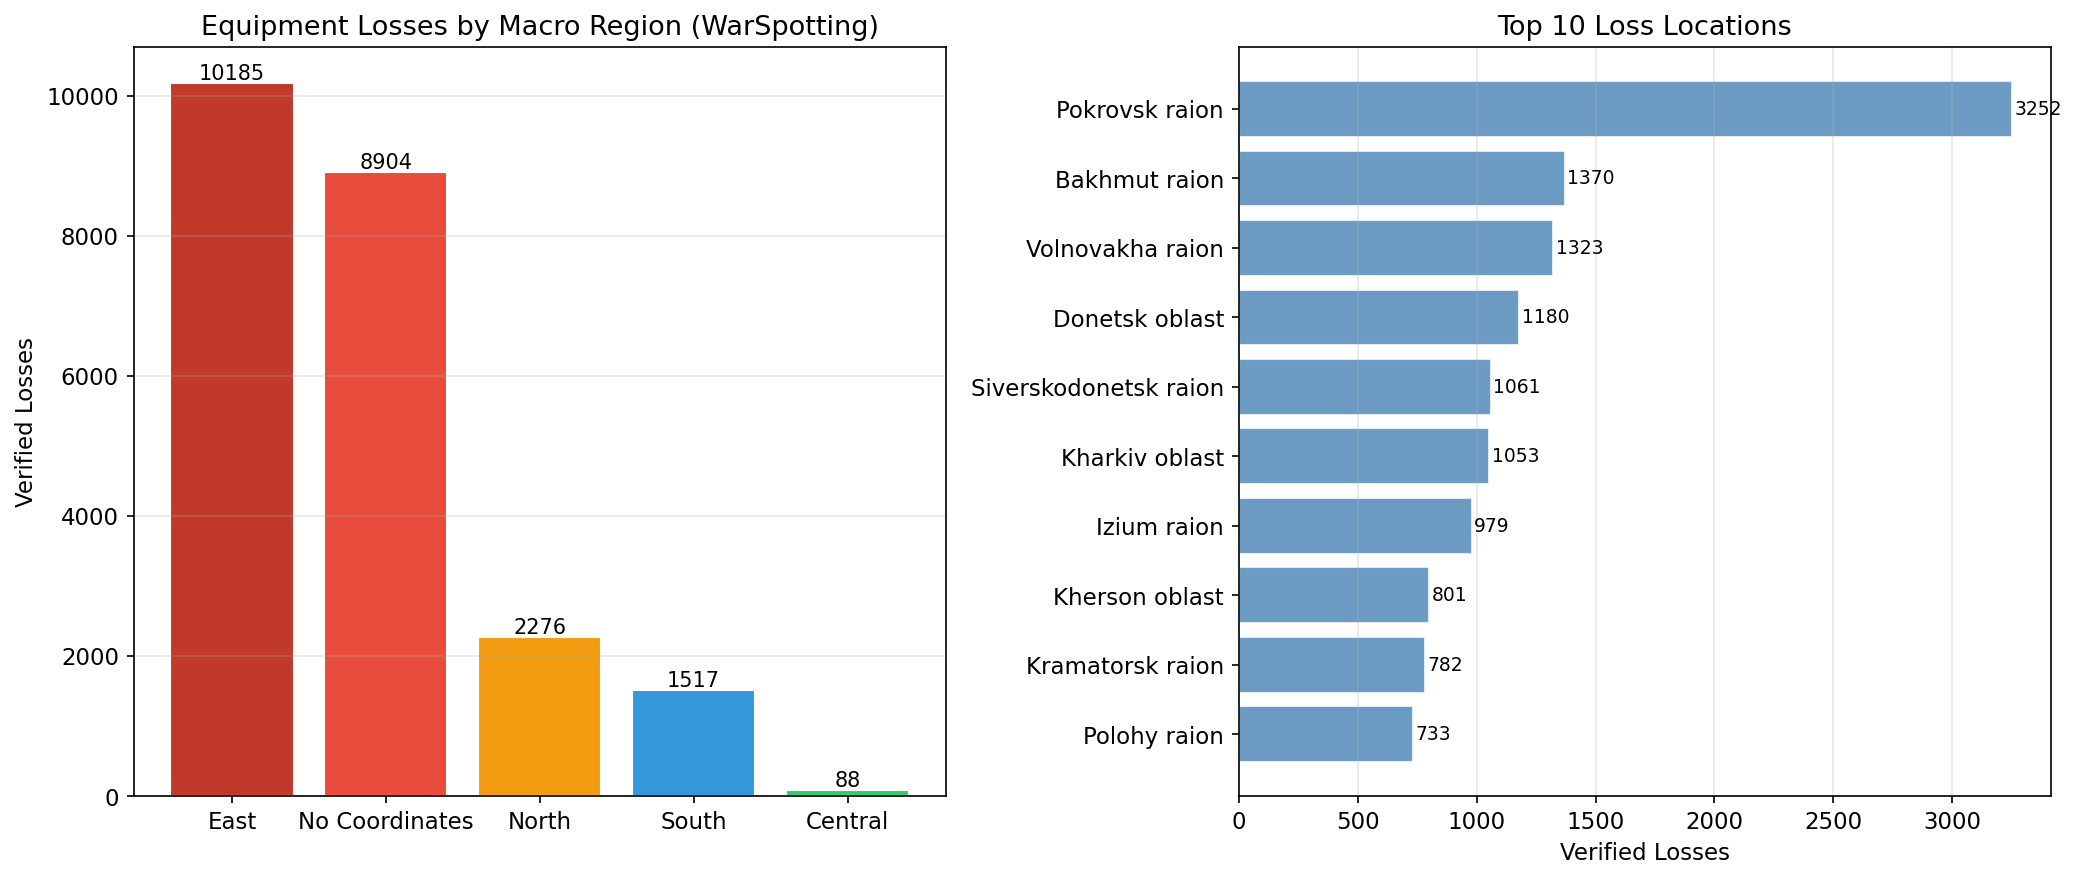
\includegraphics{../output/figures/14_spatial_distribution.png}
\caption{Spatial distribution of Russian equipment losses in WarSpotting.}
\label{fig:spatial}
\end{figure}

\subsection{Weekly Bootstrap Check}

Weekly aggregation provides an additional robustness check.

\begin{longtable}{lrr}
\toprule
Metric & Daily block bootstrap & Weekly bootstrap \\
\midrule
\endhead
Bootstrap SE & 0.9868 & \textbf{0.8212} \\
Percentile 95\% CI & [12.82, 16.59] & [13.15, 16.37] \\
BCa 95\% CI & [13.18, 17.29] & [13.31, 16.61] \\
BCa $z_0$ & 0.2211 & 0.0386 \\
BCa $a$ & 0.0222 & 0.0406 \\
\bottomrule
\end{longtable}

The weekly bootstrap standard error is still much larger than the IID bootstrap estimate. This confirms that the uncertainty inflation caused by temporal dependence is not an artifact of daily frequency. Figure~\ref{fig:weekly} shows the weekly-bootstrap distribution.

\begin{figure}[htbp]
\centering
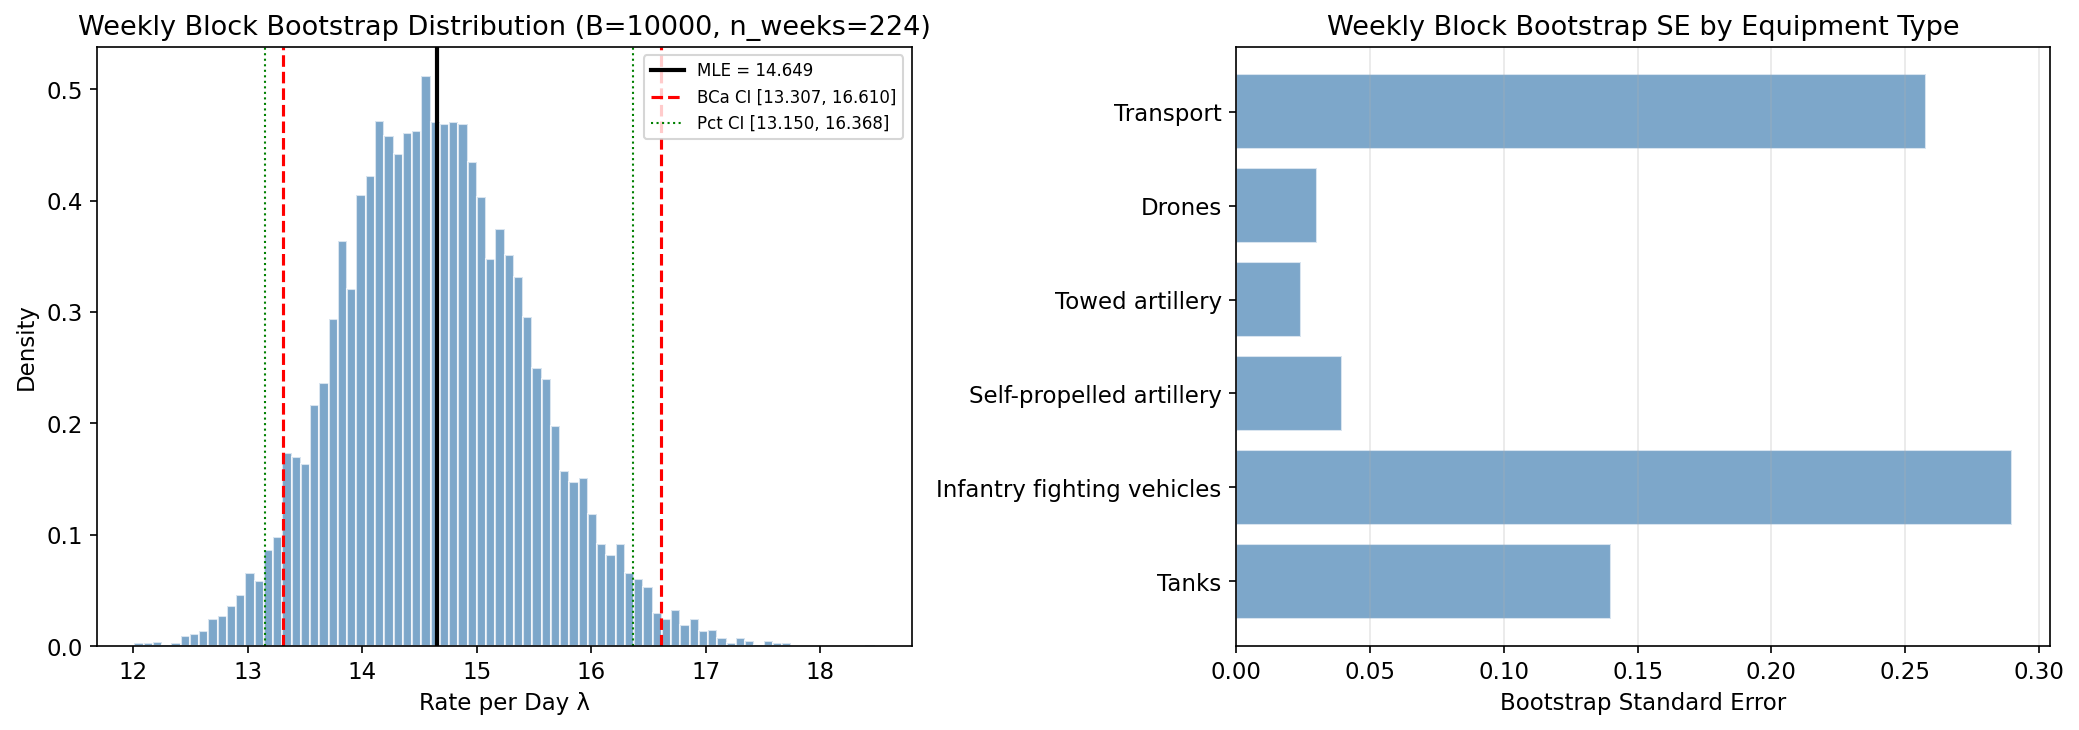
\includegraphics{../output/figures/16_weekly_bootstrap.png}
\caption{Weekly block-bootstrap distribution and BCa interval.}
\label{fig:weekly}
\end{figure}

\clearpage

\section{Discussion}

\subsection{Methodological Implications}

First, exact Poisson intervals are preferable for rare equipment categories because Wald intervals under-cover at small rates.

Second, temporal dependence is substantial in conflict data, so IID bootstrap or simple asymptotic standard errors can be misleadingly small.

Third, exact conditional tests provide a robust method for comparing two Poisson rates without relying entirely on large-sample approximations.

Fourth, observation-probability bias is not a nuisance detail; it is central to any fair comparison of visually verified conflict losses.

\subsection{Limitations}

The main limitation is that observation probabilities are not identified from Oryx alone. The bias-corrected results depend on prior assumptions about $p_{RU}$ and $p_{UA}$.

The Poisson model is also a first-order approximation; real conflict data may be overdispersed, phase-dependent, and spatially clustered. Finally, Oryx bilateral data and WarSpotting item-level records use related but not perfectly identical classification conventions.

\subsection{Future Work}

Future work could use Bayesian hierarchical models to integrate multiple sources, including Oryx, official claims, satellite imagery, and other OSINT sources.

Negative-binomial or generalized Poisson models could handle overdispersion. Spatiotemporal point-process models could explicitly model front-line movement, battle intensity, and local autocorrelation.

The estimates in this paper can also serve as inputs for forecasting models of equipment attrition.

\section{Conclusion}

Using bilateral Oryx visually verified equipment-loss records, this paper estimates daily loss rates of 15.11 items per day for Russia and 7.31 items per day for Ukraine. The observed rate ratio is 2.07 with a narrow 95\% confidence interval of [2.02, 2.11], and an exact two-Poisson conditional test rejects equal rates at $p<0.0001$.

However, the observed Oryx ratio is not automatically a true loss ratio because observation probabilities differ across sides, territory, equipment types, and time. Under a prior-based observation-bias sensitivity analysis, the corrected ratio has a median of 1.63 and a wide 95\% interval of [0.67, 3.44], with 88.1\% of bootstrap-prior draws remaining above 1.

The main conclusion is therefore directional and conditional: visually verified data strongly indicate higher Russian verified loss rates, but fair inference requires explicit reporting of uncertainty and observation-bias sensitivity.

\section*{References}

\begin{enumerate}
  \item Zammit-Mangion, A., Dewar, M., Kadirkamanathan, V., and Sanguinetti, G. (2012). Point process modelling of the Afghan War Diary. \textit{Proceedings of the National Academy of Sciences}, 109(31), 12414--12419.
  \item arXiv:2509.07813. Forecasting Russian Equipment Losses in the Ukraine War: A Multi-Model Comparison.
  \item arXiv:2408.14940. Bayesian Spatio-temporal Hawkes Process Modeling of Armed Conflict Events.
  \item Garwood, F. (1936). Fiducial limits for the Poisson distribution. \textit{Biometrika}, 28(3/4), 437--442.
  \item Krishnamoorthy, K., and Thomson, J. (2004). A more powerful test for comparing two Poisson means. \textit{Journal of Statistical Planning and Inference}, 119(1), 23--35.
  \item Efron, B., and Tibshirani, R. J. (1993). \textit{An Introduction to the Bootstrap}. Chapman \& Hall/CRC.
  \item Davison, A. C., and Hinkley, D. V. (1997). \textit{Bootstrap Methods and their Application}. Cambridge University Press.
  \item Oryx. (2022--2026). Attack on Europe: Documenting Russian and Ukrainian Equipment Losses During the Russian Invasion of Ukraine. \url{https://www.oryxspioenkop.com}
  \item leedrake5. (2022--2026). Russia-Ukraine Equipment Loss Tracking (Oryx Scraper). \url{https://github.com/leedrake5/Russia-Ukraine}
  \item WarSpotting. Automated visual identification of military equipment losses. \url{https://warspotting.net}
\end{enumerate}

\end{document}
